%%%%%%%%%%%%%%%%%%%%%%%%%%%%%%%%%%%%%%%%%%%%%%%%%%%%%%%%%%%%%%%%%%% 
%
% UMR LaTeX Thesis and Dissertation Format File, version 1.0
% Created by James Friend, UMR
% 3/3/98
%
% If you change these files, RENAME THEM!
% 
% This file is a part of the UMR thesis package.  If you
% didn't receive all the other files, complain!
%
% For documentation, look in the docs directory, and look
% around in the files.  Sorry, LaTeX isn't easy to learn or
% use, but picking up a copy of LaTeX, A Document Preparation
% System by Leslie Lamport from the bookstore might help.
%
% If you find you can't do something unusual with this format,
% there might be a "package" in the packages directory to
% help you out.  For example, lgrind for generating nice
% program code listings.
%
% If you need to change something in the format and have
% huevos, you can try modifying the umrthsis.cls file.
%
% If you don't know the formatting rules for your thesis or
% references, see your school's Graduate Studies Assistant
% or the Writing Center in H/SS.
% 
%%%%%%%%%%%%%%%%%%%%%%%%%%%%%%%%%%%%%%%%%%%%%%%%%%%%%%%%%%%%%%%%%%% 

\documentclass[chap]{mstthesis2}

\usepackage{mathrsfs,textcomp}
\usepackage{epsfig,subfigure,colordvi,graphicx}
\usepackage[all]{xy}
\usepackage[dvips]{pstricks}
\usepackage{longtable}

\newcommand {\remline} {\vspace{-12pt}}
%%% apmk: Array path marker command.
%%% We use this to indicate which elements we are talking about in an array.
\newcommand{\apmk}[1]{\Red{{#1}^\star}}
%%% The signum function
\newcommand{\sgn}{\mathrm{sgn}}
%%% Hermann Zapf's ``Chancery'' font: one of my favorites.
\DeclareMathAlphabet{\mathpzc}{OT1}{pzc}{m}{it}

% Use the first command below if you want captions over 1 line indented. A side
% effect of this is to remove the use of bold for captions. To restore bold,
% also include the second line below.
\usepackage[hang]{caption2}  
% change the caption delimiter in caption2.sty from a colon to a period:
\renewcommand\captionlabeldelim{.}

% The following command will specify the correct graphics driver for the
% graphics routines used with LaTeX.  Possible options include:
% template, dvips, oztex, textures, dvialw, emtex, dvilaser, psprint,
% dvipsone, dvi2ps, pctexps, pctex32, pctexwin, pctexhp, pubps,
% dviwin, dvitops, ln, dvipsnames.
%\ExecuteOptions{textures}
\ExecuteOptions{dvips}

\begin{document}
% Leave the following lines alone:
\addtocontents{toc}{\hfill Page}%for "Page" at top of TOC 
\addtocontents{lof}{\noindent Figure \hfill Page}%for the Figures page
\addtocontents{lot}{\noindent Table \hfill Page}%for the Tables page
\addtocontents{loa}{\noindent \hspace{1.5em}Algorithm \hfill Page}%for the Algorithms page
\addtocontents{los}{\noindent \protect\makebox[1in][l]{Symbol} Description \hfill Page}%for the Symbols page
%

%%%%%%%%%%%%%%%%%%%%%%%%%%%%%%%%%%%%%%%%%%%%%%%%%%%%%%%%%%%%%%%%%%% 
%                                                                 %
%                            TITLE PAGE                           %
%                                                                 %
%%%%%%%%%%%%%%%%%%%%%%%%%%%%%%%%%%%%%%%%%%%%%%%%%%%%%%%%%%%%%%%%%%% 
    
% Supply information for use on title page:
%   
% Title of thesis:
\thesistitle{\vskip .75in A Time Series Classifier}
% Your full name:     
\author{Christopher Mark Gore}
% The degree (Master of Science, Doctor of Philosophy, etc.): 
\degree{Master of Science}        
% Academic department:
\department{Computer Science}
% Type of thesis:       
\thesistype{1}     %=1 ->  Master's
                   %=2 ->  PhD      
% Your esteemed advisor:
\thadviser{Daniel R. Tauritz}  
% If you have a co-advisor, enter the name in the 
% curly braces below.  Otherwise, leave blank.
%\cothadviser{} % If you have 2 thesis advisers
% Committee members.
% The master's program requires two, the PhD five:
\memberone{Ralph W. Wilkerson}
\membertwo{Ray Luechtefeld}
%\memberthree{Three}
%\memberfour{Peter Parker}
%\memberfive{Uneducated}
% Graduation date.  NOT your submission date!   
\graddate{2008}
%\graddate{--- WORKING DRAFT COPY --- \timestamp\ ---}
% Copyright date below.
% If omitted, the current year is used.        
\copyrightyear{2008}
% Print titlepage and other prefatory material:
%    
\titlepage    
% Prints a copyright page, which is optional.
\copyrightpage         % optional           
% However, if you don't have a copyright page,
% print a blank page with the commands commented out
% below.
% Blank page:
%\thispagestyle{empty}
%\vspace*{1in}
%\vfill\eject

%  End of file
   % title page material

%\begin{doublespace}
\specialhead{Abstract}

% An abstract answers the following questions:

% 1. What is the problem you are solving?
A time series is a sequence of data measured at successive time intervals.
Time series analysis refers to all of the methods employed to understand such data, either with the purpose of explaining the underlying system producing the data or to try to predict future data points in the time series.
Time series analysis is applicable to many problems since there are so many areas that require a more thorough understanding of a time series or the prediction of future values of the time series.
The most typical historical examples of time series would be the weather and the financial markets but there are many more real-world time series problems.

% 2. What is your approach?
An evolutionary algorithm is a non-deterministic method of searching a solution space, and modelled after biological evolutionary processes.
A learning classifier system (LCS) is a form of evolutionary algorithm that operates on a population of mapping rules.
We introduce the time series classifier \emph{TSC}, a new type of LCS that allows for the modeling and prediction of time series data, derived from Wilson's XCSR, an LCS designed for use with real-valued inputs.
Our method works by modifying the makeup of the rules in the LCS so that they are suitable for use on a time series.
All of the operations (mutation, crossover, etc.) applied to the rules also were changed from their traditional forms.

% 3. What are your results (or expected results in some cases)?
We tested TSC on real-world historical stock data.
The system would always return a profit, but not as much as the stock market itself is capable of returning by the utilization of an indexing fund.
The stock market is a notoriously difficult system to model effectively and therefore any positive results at all are notable, and never losing money in the long-term is impressive in itself, often a difficult task for unskilled human traders.

% 4. What is the significance of the work?
Although this initial system appears incapable of producing monetary returns better than that of the stock market itself and may not be the eventual solution, it does perform well enough to demonstrate that the system is capable of learning in a very complex environment.
The inherent complexity of the market makes the system unusable for automated trading, but this approach should prove to be useful in other less challenging real-world time series problems.
     % abstract page
\specialhead{Acknowledgments}

I would like to thank for all of their support and help my parents Charles and Carolyn Gore, my wife Monica, and my advisor Daniel Tauritz.

\begin{center}
   \Cross
\end{center}
     % acknowledgments page
\tableofcontents     % table of contents (automatically generated)
\listoffigures       % required if there are figures (automatically generated)
\listoftables        % required if there are tables (automatically generated)
\renewcommand{\listofalgorithms}{%
   \listof{algorithm}
   {\thispagestyle{myheadings}%
      \pagestyle{myheadings}%
      \textbf{\listalgorithmname}%
      \addcontentsline{toc}{chapter}{\listalgorithmname}}}
\listofalgorithms

%\nomenclature        % required if there are variables (automatically generated
                     % if you use the \symbol command)

% Leave the following line alone:
\addtocontents{toc}{\parindent0pt\vskip12pt SECTION} %toc entry

\section{Introduction}

This thesis considers applying learning classifier systems (LCS's) to the prediction of time series data.
A time series as used here is a sequence of data successively measured through time.
Time series analysis encompasses many methods that attempt to understand such time series, aimed at either understanding the underlying theory present in the data points or to make real-world predictions.
Time series prediction is the use of a model to predict future events based on known past events: to predict future data points before they are measured.
One standard example is the opening price of a share of stock based on its past performance.

%\vspace*{-\baselineskip}    %You need to place this before a 
                            %subsection if it immediately follows
                            %section.
\subsection{Motivation}
No LCS to date has been designed for time series data but instead they were generally limited to Markov systems lacking any memory, which we viewed as a major limitation of LCS's.
LCS's are designed specifically with the concept of evolving an effective rule set for a specified problem, which is specifically the sort of capability that would be desirable for time series analysis and prediction: generating useful rule sets.

An LCS is an evolutionary algorithm that operates on a population comprised of rules referred to as the rule set: this rule set is used to attempt to classify a situation.
The first LCS was created by Holland \cite{HollandLCS} shortly after he created genetic algorithms (GA's) \cite{HollandGA}, one of the classical types of evolutionary algorithms.
Holland's first LCS originally used a GA as the evolutionary device.
Our system as described here also uses a GA for evolution, although it has been modified from the original form.

Holland's original LCS was quite complicated and failed to produce quality results for most real-world problems.
Because of this, the study of LCS's was somewhat inactive until Wilson introduced ZCS \cite{WilsonZCS}, a re-imagining of Holland's original LCS distilled to its most basic elements.
Wilson's ZCS was capable of producing acceptable results on certain problems and was simple enough to easily understand, reinvigorating LCS research.

A few years after introducing ZCS, Wilson modified it introducing XCS \cite{Wilson1995XCS}, which is currently one of the best performing and most popular LCS types.
Wilson's XCS was based on ZCS but with several important modifications mostly aimed at improving the accuracy of the rules produced and also for a more full coverage of the problem space by the rules.
A significant portion of the LCS's being worked on today are modifications or enhancements of Wilson's XCS.

One such enhancement of XCS is known as XCSR \cite{WilsonXCSR}, which was also developed by Wilson.
XCSR improves upon XCS by allowing it to operate with real-valued ranges for input instead of on the traditional ternary alphabet so common to LCS's, consisting of \emph{true}, \emph{false}, and a covering symbol (usually represented as $\#$ or $*$).

\subsection{Background}
The system presented here is derived from Wilson's XCSR, which is an extension of Wilson's XCS, which in turn was derived from Wilson's ZCS.
ZCS, XCS, XCSR, and this system are all learning classifier systems (LCS's), a crossover of the fields of evolutionary computation (EC) and reinforcement learning (RL), both of which are quite large fields on their own.
We will describe in this section the previous works this system was built upon.

\subsection{Reinforcement Learning}
Reinforcement learning \cite{SuttonBarto:1998a} is the process of learning how to map situations to actions to maximize a numerical reward.
The learning system is not told which actions to take, as in most forms of machine learning, but instead must discover which actions yield the most reward by exploration.
In the most interesting and challenging cases, actions may affect not only the immediate reward but also the next situation and, through that, all subsequent rewards.  
The two primary distinguishing characteristics of reinforcement learning are:
\begin{enumerate}
\item trial-and-error search and
\item delayed reward.
\end{enumerate}
Reinforcement learning is defined not by characterizing learning methods, but by characterizing a learning problem.
We consider any method that is well suited to solving that problem to be a reinforcement learning method.
The idea is to capture the most important aspects of the problem facing the learning agent interacting with its environment to achieve its goal.
Such an agent must be able to:
\begin{enumerate}
\item perceive the state of the environment,
\item act on the environment, and
\item have a goal or goals relating to the state of the environment.
\end{enumerate}
Tersely put: \textit{sensation}, \textit{action}, and \textit{goal}.

\subsubsection{Exploration versus Exploitation}
A primary challenge is the trade-off between exploration and exploitation.  A reinforcement learning agent will prefer actions that it has tried in the past and found to be effective in producing reward in order to reliably obtain more reward.  But to discover such actions, it has to try actions that it has not selected before.  The agent has to \textit{exploit} existing knowledge to obtain reward, but it also must \textit{explore} to make better action selections in the future.  Neither exploration nor exploitation can be pursued exclusively without failure.  The agent must try a variety of actions and progressively favor those that appear to be best.  On a stochastic task, each action must be tried many times to gain a reliable estimate of its expected reward.

\subsubsection{The Whole Problem}
Reinforcement learning explicitly considers the whole problem of a goal-directed agent interacting with an uncertain environment,  starting with a complete, interactive, goal-seeking agent, instead of considering subproblems without addressing how they might fit into a larger picture.  All reinforcement learning agents have explicit goals, can sense aspects of their environments, and can choose actions to influence their environments.  From the beginning, the agent operates with significant uncertainty about its environment.  For learning research to make progress, important subproblems have to be isolated and studied, but they should be subproblems that play clear roles in complete, interactive, goal-seeking agents, even if all the details of the complete agent cannot yet be filled in.


\subsection{Evolutionary Algorithms}
In artificial intelligence (AI), evolutionary algorithms (EA's) are a style of generic population-based meta-heuristic optimization algorithms whose processes are inspired by those of natural biological evolution.
The primary mechanisms employed in EA's to evolve a population of possible solutions towards an optimal one are:
\begin{enumerate}
\item parent selection based on fitness,
\item recombination,
\item mutation, and
\item and survivor selection based on fitness.
\end{enumerate}
Evolution serves as a powerful metaphor and demonstrates great creativity in both the natural world and in the world of computer science.

In normal biological evolution the environment that the population exists in exerts various pressures on the individuals in the population that determines the likelihood that any particular individual will manage to survive long enough to reproduce, and it is through this process that the fitness of an individual in the population must be determined: relative to its environment.
In an EA, the environment relates to the problem we wish to solve, the individuals in the population encode potential solutions to that problem, and their fitness is their quality as a solution to the problem.
By mimicking the methods of natural evolution in this manner we can often arrive at good solutions.
The basic evolutionary process is outlined in Algorithm~\ref{alg:evolution}.

\begin{algorithm}[H]
\caption{The evolutionary process.}
\begin{algorithmic}[1]
\label{alg:evolution}
\STATE
Initialize the population, either with randomly-generated or seeded candidate solutions or both.
\STATE
Evaluate the fitness of each member of the population.
\REPEAT
  \STATE
  Select members of the population to act as parents.
  This is typically related to the relative fitness of the parents in some way.
  \STATE
  Recombine the genetic material of the parents, producing offspring to be added to the population.
  \STATE
  Mutate some or all of the newly-created offspring.
  \STATE
  Evaluate the fitness of the offspring.
  \STATE
  Select survivors from the current population or a subset thereof, often only the newly-created offspring, to survive to the next generation.
\UNTIL{some specified termination condition is satisfied.}
\end{algorithmic}
\end{algorithm}


\subsubsection{Learning Classifier Systems}
A learning classifier system is a type of EA in which a description of a current situation is used in an attempt to map that description to some classification or action.
This is achieved through simulated evolutionary processes, where the population being evolved consists of various rules;
our entire population forms a rule set, and we apply concepts from Darwinism to our individual rules.
This is known in learning classifiers as the \emph{Michigan approach} \cite{EibenSmith}.
The other primary method employed, where each individual is an entire solution, and therefore a whole rule set, is known as the \emph{Pittsburgh approach}.
We use a modification of XCSR here, which uses the Michigan approach, and therefore so do we.

\subsubsection{ZCS}
\index{ZCS}
ZCS is a \emph{zeroth level classifier system} originally proposed in \cite{WilsonZCS}.
ZCS preserves most of the functionality of traditional LCS's, but it is a very simplified version, which aids in the understanding of the classifier and its actions.
This was a very useful contribution, because many of the problems with LCS's before then were their overly complex and detailed nature.
A good short summary of ZCS can be found in
\cite{EibenSmith}, and this summary is based primarily on that.
The basic structure of ZCS is graphically illustrated in Figure~\ref{fig:zcs}.

In ZCS there is no message list, a much-welcomed simplification of the traditional LCS.
This comes with a cost: there is no explicit method for transmitting information between cycles without the message list.
This makes the interface entirely dependent on the interface of the system with its environment, and thus assumes a Markov process.
This is most definitely an invalid assumption for real-world traded markets and for other time-series data.

\begin{figure}
\begin{center}
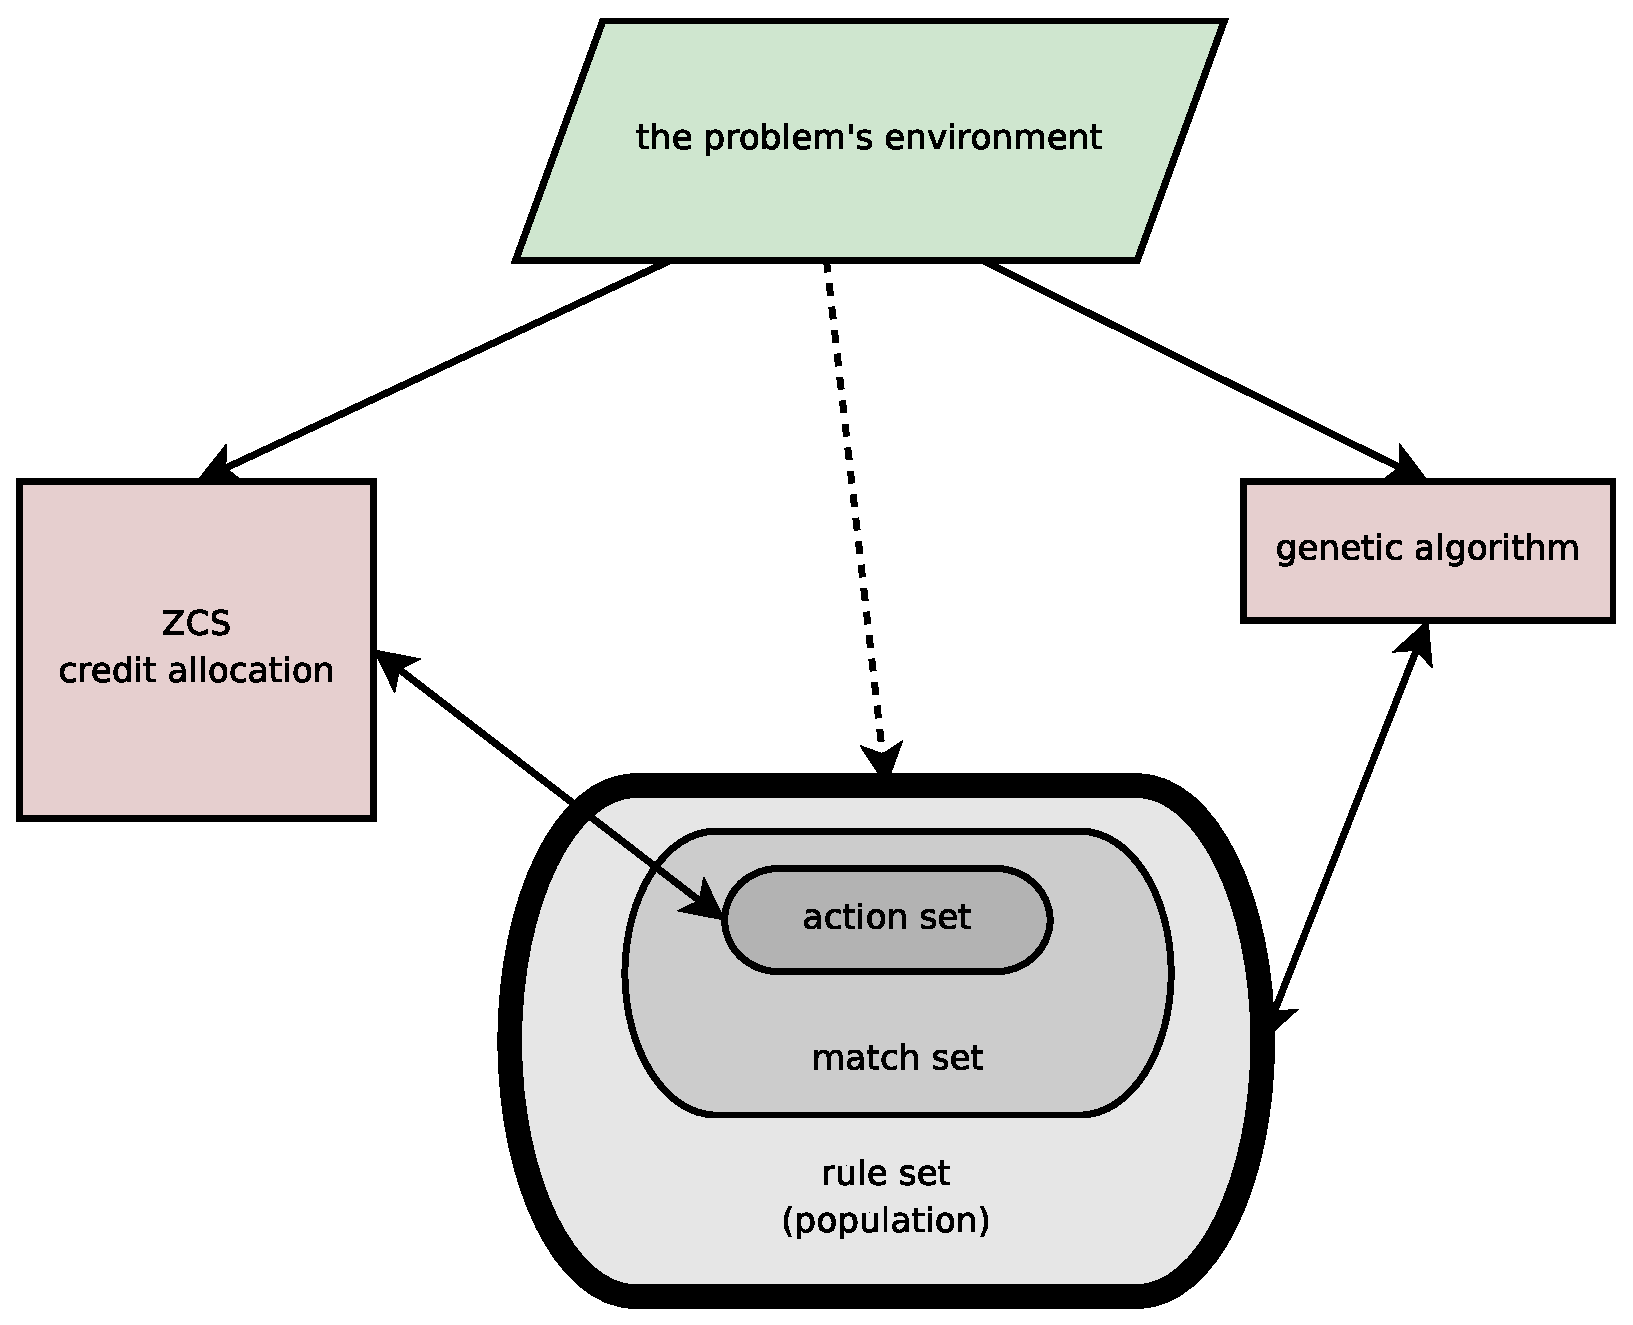
\includegraphics[width=4in]{zcs-basic-diagram.eps}
\caption{ZCS's basic structure}
\label{fig:zcs}
\end{center}
\end{figure}

Each rule $r$ is of the form $r = (c, a, s)$ where:
\begin{itemize}
\item
$c$ is the condition matched by the rule $r$ and is comprised of elements from some alphabet, typically $\{0, 1, \#\}$,
where \# is the matching symbol, matching both 0 and 1;
\item
$a$ is the action that the rule $r$ recommends;
\item
and $s$ is the real-valued strength measurement of the rule $r$, $s \in \mathbb{R}$, which determines how much of a vote rule $r$ has in selecting the action to pursue.
\end{itemize}

In each time cycle $t$ the match set $M_t$ is found, a subset of the population,
$M_t \subseteq P$,
with $P$ being the entire population of rules, the rule set.
\index{population}
\index{P@$P$|see{population}}
The members at time cycle $t$ of the match set $M_t$ can be divided into disjoint subsets based on the action they recommend.
With a finite set of possible actions
\begin{equation}
\mathpzc{A} = \{a_0, a_1, \ldots, a_{|\mathpzc{A}|}\}
\end{equation}
and $\mathpzc{A'} \subseteq \mathpzc{A}$ where
\begin{equation}
\mathpzc{A'} = \{a'_0, a'_1, \ldots, a'_{|\mathpzc{A'}|}\}
\end{equation}
comprises all of the actions represented in the match set $M_t$.
For any specific action $a'_i$ represented in the match set $M_t$ we can form the set of all members of the match set that recommend action $a'_i$, represented as
$M_{t,a'_i} \subseteq M_t$ with
\begin{equation}
M_{t,a'_i} = \left\{ r \colon r \in M_t \land a_r = a'_i \right\}.
\end{equation}
The fitness of an action $a'_i \in \mathpzc{A'}$ is then
\begin{equation}
\mathrm{fitness}(a'_i) = \sum_{\forall r \in M_{t,a'_i}} s_r,
\end{equation}
the sum of the fitness of all of the rules $r$ that recommend that particular action present in $M_{t,a'_i}$.
The action to take is selected in a fitness-proportionate method,
choosing the action $a'$ with the greatest fitness.
If $M_t = \emptyset$ then covering must take place;
a random rule that matches the current situation is created by initially setting $c$ to exactly the current situation and then replacing a few elements of $c$ at random with the \# symbol, and that suggests a randomly-selected action.

The credit assignment scheme used by ZCS is somewhat involved, and is referred to as an \emph{implicit bucket brigade}.
It attempts to reward sequences which lead to reward from the environment and which are short.
First, the rules in the population $P$ but excluded from the match set $M_t$ are originally unchanged:
\begin{equation}
s'_r = s_r \forall r \notin M_t.
\end{equation}
Next, the rules in the match set $M_t$ but excluded from the action set $A_t$
(those advocating weaker actions than the one chosen)
have their strengths reduced by a factor $\tau \in [0,1)$:
\begin{equation}
s'_r = \tau s_r \forall r \in M_t \setminus A_t.
\end{equation}
Then the strength of the rules in the current action set $A_t$ have a fraction
$\beta \in [0,1)$
of their strengths transferred to the members of the previous action set $A_{t-1}$,
reduced by a factor $\gamma \in [0,1)$:
\begin{equation}
s'_r = (1-\beta) s_r \forall r \in A_t,
\end{equation}
\begin{equation}
   s''_r = s'_r +
   \frac{\gamma \sum_{\forall r \in A_t} \beta s_r}{|A_{t-1}|}
   \forall r \in A_{t-1}.
\end{equation}
Finally, any feedback $P_t$ from the environment is reduced by $\beta$ and distributed to the rules in the current action set $A_t$:
\begin{equation}
s'''_r = s''_r + \frac{\beta P_t}{|A_t|} \forall r \in A_t.
\end{equation}

A mostly standard GA is run on the population (the rule set) periodically, with parent selection directly related to $s$ and death selection inversely related $s$.
The new rules are usually assigned the mean of their parents' strength initially.


\newpage
\subsubsection{XCS}
\index{XCS}
ZCS has many positive features, especially its simplicity and the benefits derived from its cooperative fitness sharing, but there are some notable drawbacks, primarily that it usually will not evolve a complete mapping of the environmental states and allowable actions to the possible rewards, often quickly selects local optima, and breeds across niches, as noted in \cite{Wilson1995XCS}.
These drawbacks led Wilson to heavily modify ZCS into what is called XCS \cite{Wilson1995XCS}.
In XCS, several of the deficiencies in ZCS are addressed.
The basic structure of XCS is graphically illustrated in Figure~\ref{fig:xcs}.

In ZCS, the GA is run on the entire population, a \emph{panmictic} approach \cite[p.~155]{EibenSmith}.
This is ineffective for most problems, so in XCS the GA was run only in the current match set at the time step that the GA is run in the initial version of XCS, and only in the current action set at the time step that the GA is run in the later variants of XCS.
We run the GA on the current action set in this work.
This allows for a more accurate rule set to be evolved, since each niche is best viewed as its own sub-problem.

In ZCS, a rule is allowed to survive by the GA on the basis of its payoff.
This is problematic,
since it biases against rules early in a chain of events that are eventually profitable,
and because rules that may be the most appropriate for an event might have a relatively low payoff.
This caused ZCS to often fail to create a complete mapping and fail to evolve accurate generalizations.
This is remedied in XCS by creating a fitness measure for the rules, separate from the predicted payoff, used by the GA.

\begin{figure}
\begin{center}
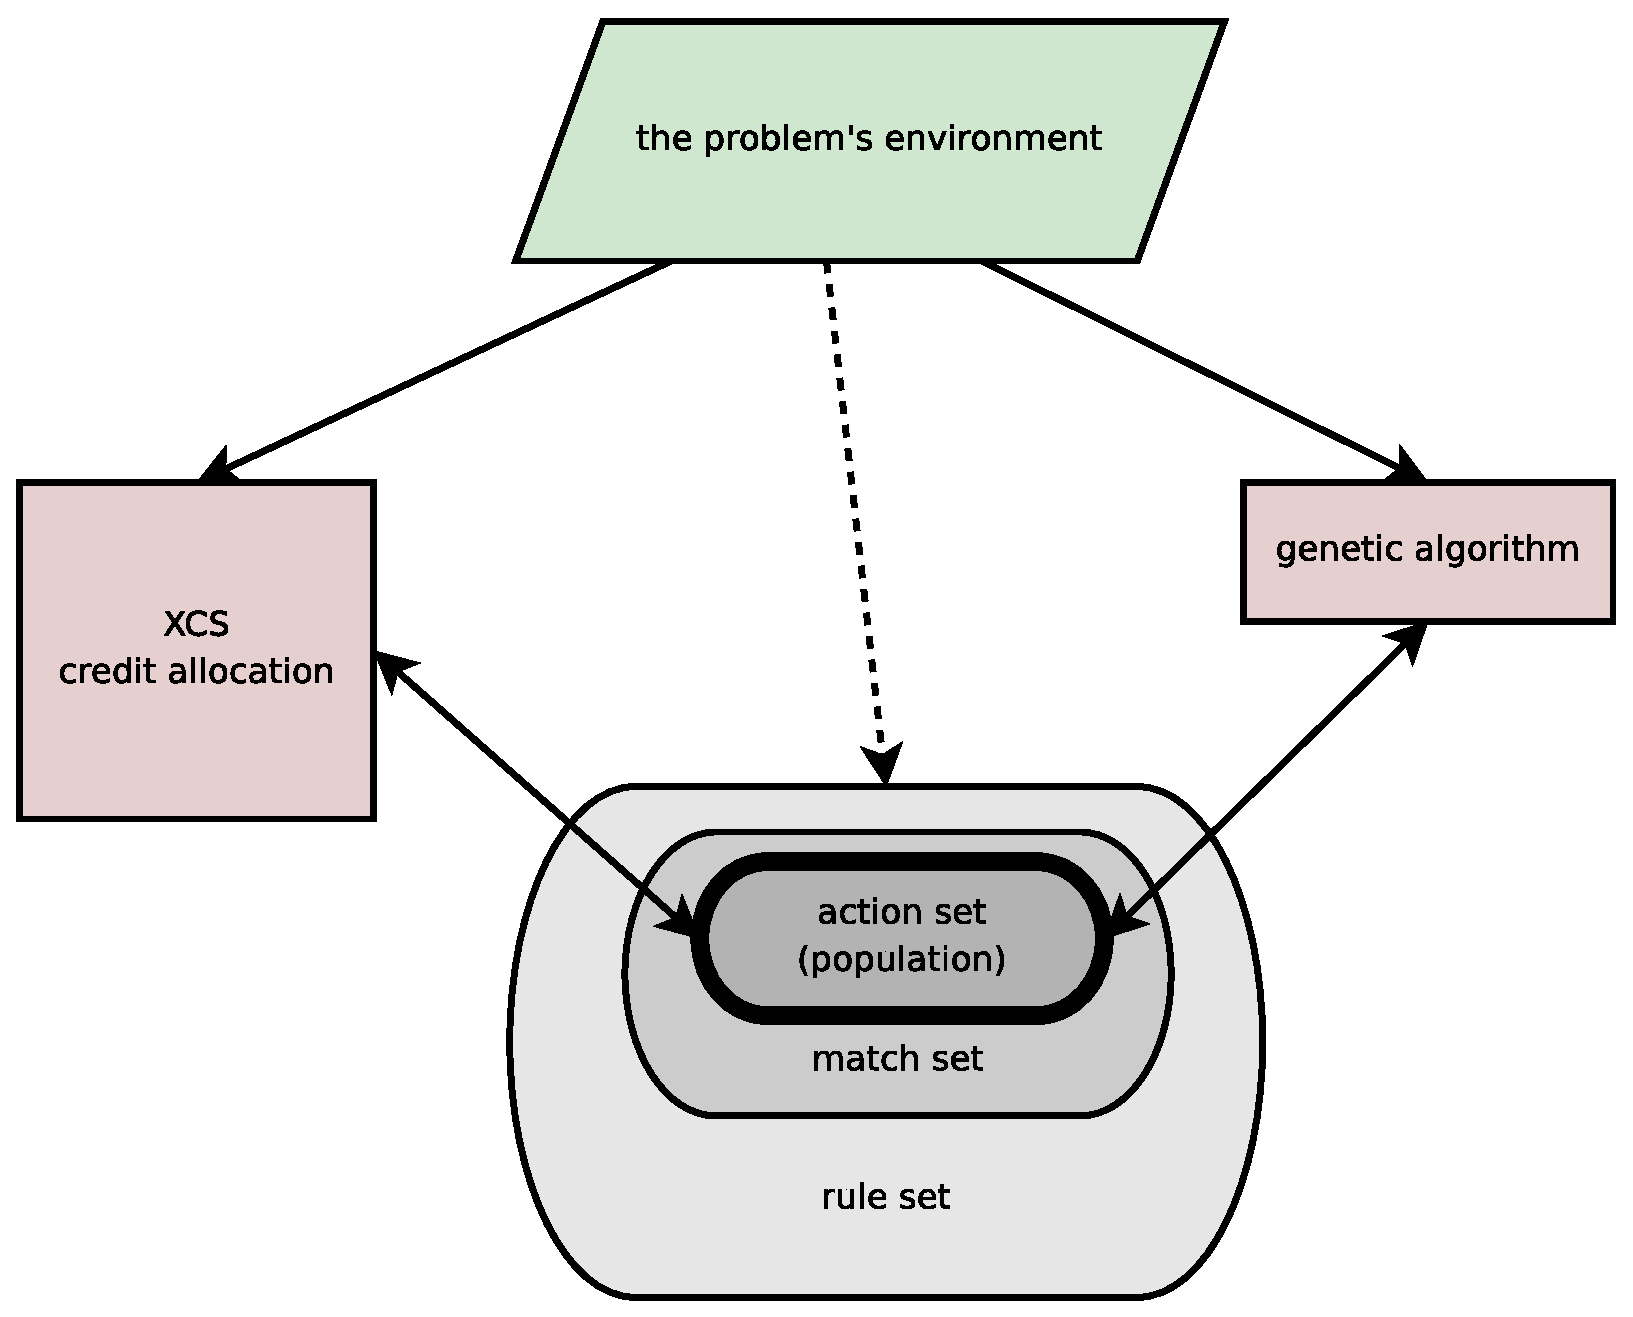
\includegraphics[width=4in]{xcs-basic-diagram.eps}
\caption{XCS's basic structure}
\label{fig:xcs}
\end{center}
\end{figure}

Each rule $r$ is now of the  more complex form
\begin{equation}
r = (c, a, p, \epsilon, F, exp, ts, as, n),
\end{equation}
where:
\begin{itemize}
\item
$c$ is the condition matched by the rule $r$, comprised of elements from some alphabet such as $\{0, 1, \#\}$,
where \# is the matching symbol, matching both 0 and 1.
\item
$a$ is the action that the rule $r$ recommends.
\item
$p$ is the predicted payoff.
\item
$\epsilon$ is an estimate of the prediction error.
\item
$F$ is the fitness used by the GA.
It is vital that the fitness used by the GA is a measure of the \emph{accuracy} of the rule,
and not a measure of the \emph{magnitude} of the rule, where the magnitude of a rule is how active that rule is in relation to the rest of the rules in the rule set, since a rule with greater magnitude but lower accuracy can be a detriment to the system.
For example, a rule that always matched every situation (all \#'s in the condition) but only accurately predicted 51\% of the situations would have high magnitude but low accuracy.
\item
$exp$ is the experience of the rule,
a count of the number of times since this classifier's creation that it has belonged to the action set.
\item
$ts$ is a time stamp of the last occurrence of a call to the GA in an action set that this classifier was a part of, as the generational number.
\item
$as$ is an estimate of the average action set size this classifier has belonged to.
\item
$n$ is the numerosity of this macro-classifier.
This is how many traditional micro-classifiers this macro-classifier represents.
Groups of entirely identical normal classifiers (the micro-classifiers) are subsumed into macro-classifiers instead of being allowed to exist separately within the rule set; this serves solely as a computational time-saver.
Therefore the only difference between a normal classifier (a micro-classifier) and a macro-classifier is the presence of the numerosity, which is a count of how many micro-classifiers that specific macro-classifier represents.
\end{itemize}


\subsubsection{XCSR}
\index{XCSR}
Wilson extended his concept of XCS with XCSR in \cite{WilsonXCSR}.
Classifier systems had typically taken strings from some small alphabet, often binary, as input until then
even though many real-world problems have input from the environment of the form $\mathbb{R}^n$ for some order $n \in \mathbb{Z}, n>0$.
Wilson's XCSR allows XCS to operate on just such an input.
XCSR is identical to normal XCS with the exception of the input interface, the nature of the predicates, the mutation operator, and the details of covering.
The basic structure of an XCSR rule is graphically illustrated in Figure~\ref{fig:xcsr-rule}.

Originally the predicates in XCSR were intervals of the form
\begin{equation}
interval_i = \{center_i,spread_i\},
\end{equation}
such that an environmental input $x_i$ was matched by $interval_i$ if and only if
\begin{equation}
center_i-spread_i \le x_i \le center_i+spread_i,
\end{equation}
but this was discovered to induce a bias \cite{StoneBull:2003}, so the representation was eventually changed to be
\begin{equation}
interval_i = \{lower_i,upper_i\},
\end{equation}
where now $x_i$ is matched by $interval_i$ if and only if
\begin{equation}
lower_i \le x_i \le upper_i.
\end{equation}
We use the $\{lower,upper\}$ form in this work.

\begin{figure}
\begin{center}
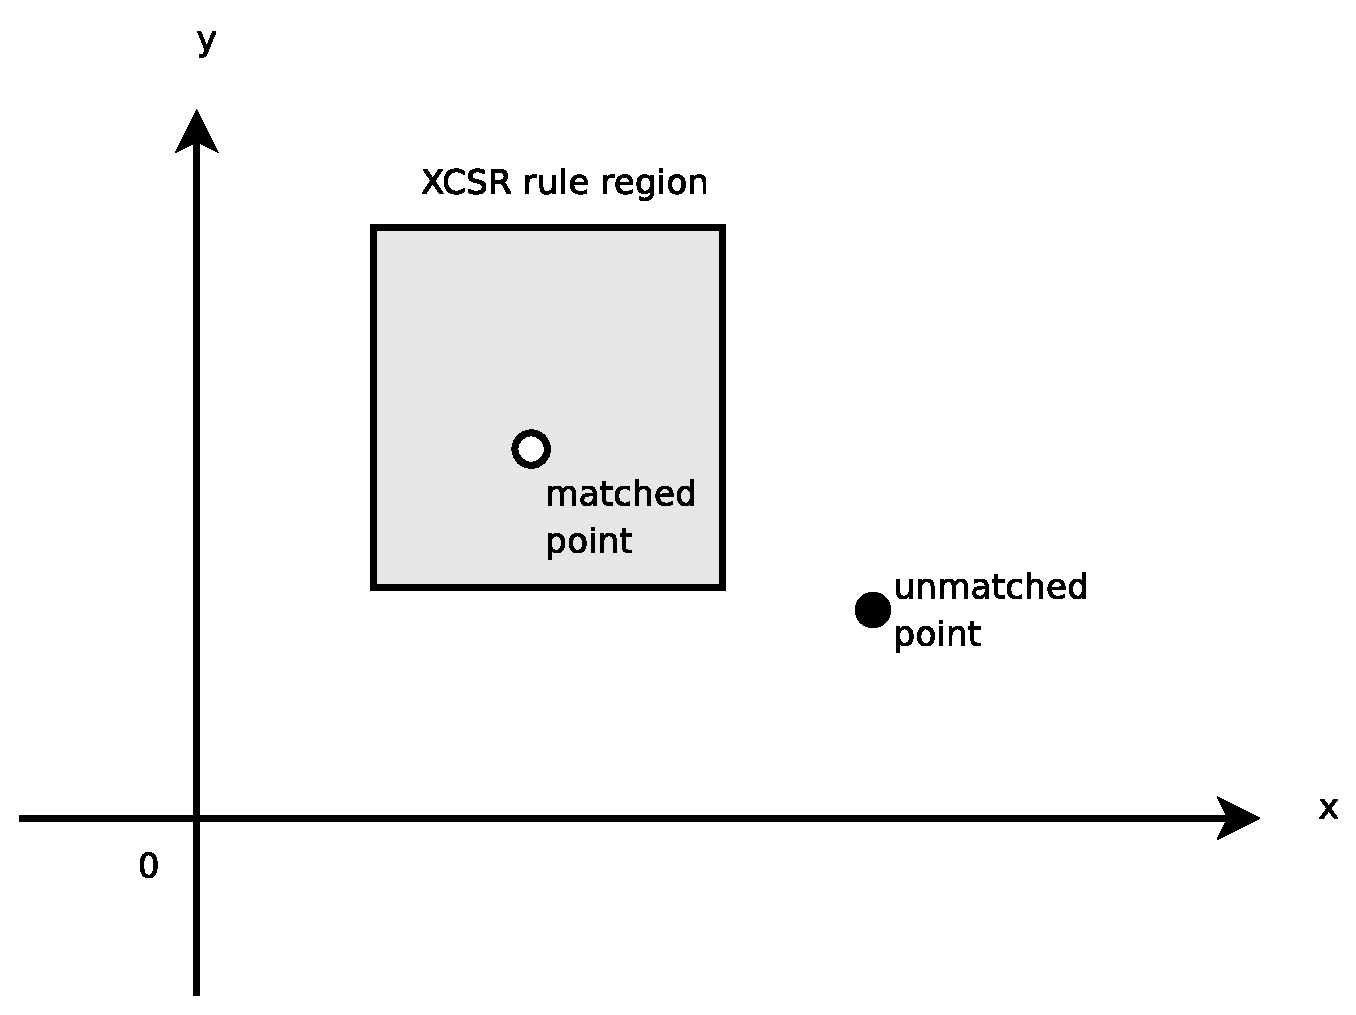
\includegraphics[width=4in]{xcsr-interval.eps}
\caption{XCSR's interval rules}
\label{fig:xcsr-rule}
\end{center}
\end{figure}

\newpage
Crossover is simple two-point crossover, but on the sequence
\begin{equation}
\{center_0,spread_0, \ldots\}
\end{equation}
or
\begin{equation}
\{lower_0,upper_0, \ldots\}
\end{equation}
depending on the predicate type,
in both cases therefore allowing the crossover points to fall within a single allele.

In the original XCSR, mutation was performed by adding a small random quantity from the range $[-0.1,0.1]$ to each allele, and all problems were to have their input scaled to $[0,1]$.
The variation of XCSR used here is capable of scaling outside of $[0.0,1.0]$, so instead mutation is performed as the addition or subtraction of a small percentage of the overall range as seen so far.



\section{Time Series Prediction}
\vspace*{-\baselineskip}

\subsection{ARIMA and Other Statistical Methods}
ARIMA, the \emph{autoregressive integrated moving average}, is a common and very powerful statistical method often used in econometric models that can help forecast and estimate what is going to happen in the future.
The ARIMA time series analysis uses lags and shifts in the historical data to uncover patterns (e.g., moving averages, seasonality) and predict the future \cite{BoxJenkins:1994}.
The ARIMA model was first developed in the late 1960s but was not systemized until the work of Box and Jenkins in 1976 \cite{BoxJenkins:1976}.
ARIMA can be more complex to use than other statistical forecasting techniques, although when implemented properly can be quite powerful and flexible.  ARIMA is a method for determining two things:
\begin{enumerate}
\item how much of the past should be used to predict the next observation (length of weights) and
\item the values of the weights.
\end{enumerate}

Three common models of time series data are \textit{autoregressive} (AR) models, the \textit{integrated} (I) models, and the \textit{moving average} (MA) models.
These three classes depend linearly on previous data points and are combined in the autoregressive integrated moving average (ARIMA) model.
A model of this form is referred to as an $ARIMA(p,d,q)$ model where $p,d,q \in \mathbb{N^*}$.
The order of the autoregressive part is $p$, the order of the integrated part is $d$, and the order of the moving average part is $q$.
Given a time series of data $X_t$ (where $t$ is integer valued and the $X_t$ are real numbers) then an $ARIMA(p,d,q)$ model is given by
\begin{equation}
\left(1 - \sum_{i=1}^p \phi_i L^i\right) (1-L)^d X_t =
\left(1 + \sum_{i=1}^q \theta_i L^i\right) \varepsilon_t\,
\end{equation}
where $L$ is the lag operator,
$\phi$ are the parameters of the autoregressive part of the model,
$\theta$ are the parameters of the moving average part,
$d \in \mathbb{N^*}$ (if instead we have $d=0$ then this model is equivalent to an ARMA model),
and the $\epsilon_t$ are error terms.
The error terms $\epsilon_t$ are generally assumed to be independent and identically distributed variables sampled from a normal distribution with zero mean:
$\epsilon_t \sim N(0,\sigma^2)$ where $\sigma^2$ is the variance.
ARIMA models are commonly used for predicting and analyzing simpler time series.
They have been used on the stock market, but are generally viewed only as an indicator, not a predictive tool, due to the complexity of the market and because of their need for accurate knowledge about the time series itself.
It is for similar reasons that most traditional statistical methods fail to be of any real use in this task.

For example
\begin{equation}
y(t)= \frac{y(t-3)}{3} + \frac{y(t-2)}{3} + \frac{y(t-1)}{3}
\end{equation}
is a potential ARIMA model; another potential ARIMA model is
\begin{equation}
y(t)= \frac{y(t-3)}{6} + \frac{4 y(t-2)}{6} + \frac{y(t-1)}{6}.
\end{equation}
The correct ARIMA model requires identification of the right number of lags and the coefficients that should be used.  ARIMA model identification uses autoregressions to identify the underling model.  Care must be taken to robustly identify and estimate parameters as outliers (pulses, level shifts, local time trends) can wreak havoc.

\subsection{Artificial Neural Networks}
An artificial neural network is a graph of connected processing elements called neurons which can exhibit complex global behavior as determined by the connections between the neurons and their parameters.
This technique was originally inspired by the examination of the central nervous systems of living creatures, most notably that of humans, the most significant information processing system found in nature.
While a neural network is not adaptive itself, most practical examples use algorithms designed to alter the weights of the connections in the network to produce a desired signal flow.
These networks are also similar to their biological counterparts in that their functions are performed collectively in parallel by the entire network, with no clear delineation of sub-tasks to which various units are assigned.
Modern artificial neural networks often abandon much of this for a more practical approach based on statistics and signal processing \cite{HK:2000:ANN}.
There have been many attempts to predict financial time series with artificial neural networks
\cite{WuLu:1993:CSC93, KR:1994:NNAPL},
and there have even been somewhat successful results using genetic algorithms to evolve the weights for neural networks \cite{SC:2002:NNGA, KCM:2005:GECCO2005}.
However, there is one main drawback that comes with the use of artificial neural networks.
There is no easy way to translate the neural network that has been produced into an understandable set of rules describing its innate knowledge: the information is effectively trapped in the weights on the neurons.
Extracting useful rules from ANN's is a challenging field unto itself \cite{AndrewsGeva:2000}.

\subsection{Non-LCS Evolutionary Approaches}
There have been attempts at using evolutionary approaches other than LCS's to predict and analyze markets and other time series, ranging from the simplistic to the very complex.
In \cite{FGLG:2006:GECCO}, traditional genetic algorithms were used to optimize the exact numbers to be used in traditional technical analysis.
In \cite{Belford:2006:GECCO}, traditional genetic algorithms were again used, but this time in optimizing the rule sets for candlestick-style analysis; this outperformed a random trader.
In \cite{Kaboudan:2000:CompEcon}, a simplified variant on the concept of genetic programming, coded in C++, was used to develop trading rules for six stocks, and they managed to return better results than both the market and a naive trader.
However, the innate challenges of the real market have lead many researchers to resort to simulated markets, whose simplicity can make fundamental discoveries about economic theory sometimes less challenging to achieve; a small survey of these sorts of markets can be found in \cite{WHD:2002:AIReview}.

\subsection{LCS-Based Approaches}
There have been a few attempts at using LCS's to analyze and predict financial markets.
We will highlight a few derived from XCS here, since the system presented here is also derived from XCS.

\subsubsection{XCS}
A predictive system lacking a memory component is almost completely useless in attempting to model a highly interdependent nonlinear multivariate time series such as the stock market with any hope of utility;
none the less, it has been attempted.
One of the more notable attempts at this is described in \cite{SchulenburgRoss:1996:LNAI}, in which an XCS was used to predict the correct trading action for a stock on consecutive trading days.
Later work by Schulenburg and Ross in \cite{SchulenburgRoss:2002:LETS} does show some promise:
they utilize the opinions of a large host of simulated traders in order to make a decision.
This would yield in the general vicinity of 9\%p.a. returns: not spectacular or applicable to real-world trading, but respectable.

\subsubsection{XCSF}
In \cite{Wilson:2001:GECCO} Wilson outlined an extension to XCS for the approximation of functions, called XCSF, which attempts to learn a function of the form $y=f(x)$,
where $y \in \mathbb{R}$, $|x|=n$, and $x_i \in \mathbb{Z} \forall x_i \in x$.
A classifier consists of $n$ interval predicates of the form $int_i = (l_i, u_i)$
and matches an input $x$ if and only if $l_i \le x_i \le u_i \forall i \in \mathbb{N}$. 
Classical two-point crossover is employed, but where crossover may occur in-between the alleles or at the ends of the prediction, although the action is not involved in the crossover process.
A covering classifier is generated for a situation $x$ by forming the $l_i$ through subtracting from $x_i$ some random integer from $[0,r_0]$, and forming $u_i$ by adding some other random integer from $[0,r_0]$ to $x_i$, both limited to a maximum range of possible input, where $r_0$ is a parameter.
A rule $r^1$ can subsume a rule $r^2$ if and only if $l^1_i \le l^2_i \land u^2_i \le u^1_i \forall i$.  
While this could possibly be used to predict some very simplistic time series data, function approximation often does not perform very well in real-world problems, as is well-known in reinforcement learning literature \cite{BoyanMoore:2004,PerkinsPrecup:2002},
and this drawback of XCSF (and similar approaches) is explicitly acknowledged in \cite{LLWG:2005:GECCO}.
This would be most definitely true of a system as complex as the stock market, which cannot be easily and usefully mapped to any polynomial.

\section{Approach and Design of the Time Series Classifier}

\vspace{-\baselineskip}

\subsection{Fundamental Operations}

Our representation of a time series and our approach to their evolutionary methods requires us to be capable of generating multi-dimensional raster paths, where a raster path is a one-dimensional path through a raster space.
This is so that we can run raster paths through a raster space of data, a discrete sampling of data.
A raster space is one that is representable by
$\mathbb{Z}_a \times \mathbb{Z}_b \times \cdots \times \mathbb{Z}_z$.
In other words, all of the dimensions are along sets of finite integers instead of the real numbers.
A common example is raster imagery: a two-dimensional bitmap of size $m \times n$ can be viewed as a complete representation of the two-dimensional raster space of $\mathbb{Z}_m \times \mathbb{Z}_n$.
A multidimensional matrix can therefore fully represent these spaces, instead of merely being samplings of the real space, although we are using these raster spaces for sampling of real data in our approach.
We form a useful sample of the data for further analysis and classification by TSC by generating paths through the data and it is these raster paths that the TSC actually classifies the situations with, not with the entire data set which is generally very large.
We will now outline the basic operations we use to generate raster lines.

\subsubsection{The \emph{Sort On} Algorithm}
\index{sort on algorithm@\emph{sort on} algorithm}
This algorithm sorts a sequence $s$ according to the ordering of another sequence $t$, and is outlined in Algorithm~\ref{alg:sort-on}.
\begin{algorithm}[H]
\caption{Sort on.}
\label{alg:sort-on}
\begin{algorithmic}[1]
\INPUT A sequence $s$ to be sorted.
\INPUT A sequence $t$ upon which to sort $s$ with.
\INPUT A comparator $c$ to sort with, typically $>$ or $<$.
\REQUIRE $|s| = n \le |t|$.
\STATE Construct a sequence $u$ containing pairs of the form $u_i = (s_i, t_i)$ as elements, $|u| = n$,
  \begin{equation}
  u = (u_0, \ldots, u_{n-1})
    = \left( (s_0, t_0), \ldots, (s_{n-1}, t_{n-1}) \right).
  \end{equation}
\STATE Sort $u$ using the second elements as the key, using any normal sorting algorithm, giving
  \begin{equation}
  u' = \left( (s'_0, t'_0), \ldots, (s'_{n-1}, t'_{n-1}) \right)
  \end{equation}
  where $t'_0 \le \ldots \le t'_{n-1}$ if we are sorting in ascending order (with the $<$ comparator).
\RETURN $s' = \left( s'_0, \ldots, s'_{n-1} \right)$.
\end{algorithmic}
\end{algorithm}

\subsubsection{The \emph{Sort Order} Algorithm}
\index{sort order algorithm@\emph{sort order} algorithm}
This algorithm returns the re-ordered indices of a sorted sequence, and is outlined in Algorithm~\ref{alg:sort-order}.
For example, if $t = \{4,5,3,9\}$
then the sorted ordering of $t$ would be $\{3,1,0,2\}$
since $t_3 \ge t_1 \ge t_0 \ge t_2$.
\begin{algorithm}[H]
\caption{Sort order.}
\label{alg:sort-order}
\begin{algorithmic}[1]
\INPUT A sequence $t$.
\INPUT A comparator $c$, usually $<$ or $>$.
\LETARROW{$n$} $|t|$.
\STATE Generate $\mathbb{Z}_n = (0, \ldots, n-1)$.
\RETURN The result of the \emph{sort on} algorithm from \S\ref{alg:sort-on} on $s = \mathbb{Z}_n$ with $t$ and the comparator $c$.
\end{algorithmic}
\end{algorithm}

%\subsubsection{The \emph{Map Inverse} Algorithm}
%\index{map inverse algorithm@\emph{map inverse} algorithm}
%This algorithm finds the inverse of a mapping, and is outlined in Algorithm~\ref{alg:map-inverse}.
%\begin{algorithm}[H]
%\caption{map inverse}
%\label{alg:map-inverse}
%\begin{algorithmic}[1]
%\INPUT A map $m \colon \mathbb{Z}_n \rightarrow \mathbb{Z}_n$, represented as a sequence.
%\STATE Validate that $m$ is a valid map.
%  Sort $m$ giving $m'$, and then remove any duplicates from $m'$ giving $m''$.
%  Check that $m'' = \mathbb{Z}_n$ where $n = |m|$.
%\RETURN $m^{-1}$, the inverse of $m$,
%  by calling the \emph{sort on} algorithm from \S\ref{alg:sort-on} with
%  $s = \mathbb{Z}_n$ and $t = m$.
%\end{algorithmic}
%\end{algorithm}

\subsubsection{Rasterized Linear Paths Through Arrays}
Given an array $A$ of rank $r$ and dimensions
$d_0 \times \cdots \times d_{r-1}$,
we wish to pull a one-dimensional list or vector $v$ of values from the array, starting at position
$A_{s_0\,\ldots\,s_{r-1}}$
and finishing at position
$A_{f_0\,\ldots\,f_{r-1}}$,
following a linear path through the array.

As an example consider the $4 \times 6$ array:
$$A = \left(\begin{array}{cccccc}
a & b & c & d & e & f \\
g & h & i & j & k & l \\
m & n & o & p & q & r \\
s & t & u & v & w & x
\end{array}\right).$$

\paragraph{A purely horizontal path.}
The linear path from $A_{0\,0}$ to $A_{0\,5}$ would be composed of the values
$$\left< A_{0\,0}, A_{0\,1}, A_{0\,2}, A_{0\,3}, A_{0\,4}, A_{0\,5} \right>$$
and would be
$$\left< a, b, c, d, e, f \right>$$
as illustrated by
$$A = \left(\begin{array}{cccccc}
\apmk a & \apmk b & \apmk c & \apmk d & \apmk e & \apmk f \\
g & h & i & j & k & l \\
m & n & o & p & q & r \\
s & t & u & v & w & x
\end{array}\right).$$

\paragraph{A purely vertical path.}
The linear path from $A_{0\,0}$ to $A_{3\,0}$ would be composed of the values
$$\left< A_{0\,0}, A_{1\,0}, A_{2\,0}, A_{3\,0} \right>$$
and would be
$$\left< a, g, m, s \right>$$
as illustrated by
$$A = \left(\begin{array}{cccccc}
\apmk a & b & c & d & e & f \\
\apmk g & h & i & j & k & l \\
\apmk m & n & o & p & q & r \\
\apmk s & t & u & v & w & x
\end{array}\right).$$

\paragraph{A traditional diagonal path.}
The linear path from $A_{0\,0}$ to $A_{3\,3}$ would be composed of the values
$$\left< A_{0\,0}, A_{1\,1}, A_{2\,2}, A_{3\,3} \right>$$
and would be
$$\left< a, h, o, v \right>$$
as illustrated by
$$A = \left(\begin{array}{cccccc}
\apmk a & b & c & d & e & f \\
g & \apmk h & i & j & k & l \\
m & n & \apmk o & p & q & r \\
s & t & u & \apmk v & w & x
\end{array}\right).$$

\paragraph{Non-equal diagonal paths.}
The confusing part arises when we are dealing with diagonal paths with unequal steps.
Consider the linear path from $A_{0\,0}$ to $A_{3\,5}$.
We end up with a stair-stepping path through the array:
$$\left(A_{0\,0}, A_{1\,1}, A_{2\,1}, A_{3\,2}, A_{4\,2}, A_{5\,3}\right)$$
and would be
$$\left(a, h, i, p, q, x\right)$$
as illustrated by
$$A = \left(\begin{array}{cccccc}
\apmk a & b & c & d & e & f \\
g & \apmk h & \apmk i & j & k & l \\
m & n & o & \apmk p & \apmk q & r \\
s & t & u & v & w & \apmk x
\end{array}\right).$$

\paragraph{The Raster Line Algorithm.}
This is the algorithm used to determine a linear raster path, and is outlined in Algorithm~\ref{alg:raster-line}.
It returns a list of points that follow the linear path from the starting point $p$ to the ending point $q$.
This is derived from the algorithm for raster conversion of a 3D line as described in \cite{KaufmanShimony1986}.
This should work for any dimensionality.
\begin{algorithm}[H]
\caption{Raster line.}
\label{alg:raster-line}
\begin{algorithmic}[1]
\INPUT a starting point $p$ and a final point $q$, both represented as lists.
\REQUIRE $|p| = |q| \land
   p_i \in \mathbb{N} \forall p_i \in p \land
   q_i \in \mathbb{N} \forall q_i \in q$.
\IF[This is a simple degenerate case.]{$p = q$}
  \RETURN $\{p\}$, a list containing only one element, $p$.
\ENDIF
\LETARROW{$n$} $|p| = |q|$ be the dimensionality.
\LETARROW{$\delta$} $\left\{ |p_0 - q_0|, \ldots, |p_{n-1} - q_{n-1}| \right\}$, $|\delta| = n$.
\LET $o$ be the sorted ordering of $\delta$ by $>$ from the \emph{sort order} algorithm in \S\ref{alg:sort-order}.
\LET $p'$ and $q'$ be $p$ and $q$ respectively, sorted according to $o$.
\IF[We want the starting point to have the lower initial dimension.]
   {$p'_0 \le q'_0$}
   \STATE Swap $p'$ with $q'$.
\ENDIF
\LETARROW{$\delta'$} $\left\{ |p'_0 - q'_0|, \ldots, |p'_{n-1} - q'_{n-1}| \right\}$.
\LETARROW{$s$} $\left( \sgn \left( p'_0 - q'_0 \right), \ldots,
   \sgn\left( p'_{n-1} - q'_{n-1} \right) \right)$,
    where $\sgn$ is the signum function.
\LETARROW{$d$} $\left\{ d_1, \ldots, d_{n-1} \right\}, |d| = n-1$,
   the deciders, where $d_i \leftarrow 2 \delta'_i - \delta'_0 \forall d_i \in d$.
\LETARROW{$a$} $\left\{ a_1, \ldots, a_{n-1} \right\}, |a| = n-1$, the if-increments, $a_i \leftarrow 2 \delta'_i \forall a_i \in a$.
\LETARROW{$b$} $\left\{ b_1, \ldots, b_{n-1} \right\}, |b| = n-1$, the else-increments, $b_i \leftarrow 2 \left( \delta'_i - \delta'_0 \right) \forall b_i \in b$.
\LETARROW{$r$} $\{ p' \}$, initializing the result of the algorithm, an ordered list of points.
\LETARROW{$z$} $p'$, initializing the current point.
\WHILE[After this, we have $r = \left\{ p', \ldots, q' \right\}$.]
  {$z_0 < q'_0$}
  \STATE Increment $z_0$ by 1.
  \FORALL{$d_i \in d$}
    \IF{$d_i < 0$}
      \STATE increment $d_i$ by $a_i$.
    \ELSE[In this case we have $d_i \ge 0$.]
      \STATE increment $d_i$ by $b_i$ and $z_i$ by $s_i$.
    \ENDIF
  \ENDFOR
  \STATE Push a duplicate of $z$ to the back of $r$, so that now $r = \left\{ p', \ldots, z \right\}$.
\ENDWHILE
\STATE  Reorder the coordinate of the points in $r$ according to the original coordinate ordering forming $r'$ by applying the inverse of $o$, which is $o$.
\IF{we originally swapped the start and end points}
  \RETURN the reverse of $r'$.
\ELSE
  \RETURN $r'$.
\ENDIF
\end{algorithmic}
\end{algorithm}

\subsubsection{List Slices}
This function returns a slice from a one-dimensional list; that is, a modular subset of the list, and is outlined in Algorithm~\ref{alg:list-slice}.
For example, a 2-slice of the list  $\{1,2,3,4,5,6,7,8,9\}$ would be the list $\{1,3,5,7,9\}$.
\begin{algorithm}[H]
\caption{List slice.}
\label{alg:list-slice}
\begin{algorithmic}[1]
\INPUT A list of elements $l = \{l_0, l_1, \ldots, l_{|l|}\}$.
\INPUT A positive rational slice size $s$.
\STATE Initialize the resulting list $r \leftarrow nil = \{\}$, initially empty.
\STATE Initialize the moving index $i \leftarrow 0$.
\WHILE{$i < |l|$}
  \IF{$i \in \mathbb{Z}$}
    \STATE Append $l_i$ to the end of $r$.
  \ENDIF
  \STATE $i \leftarrow i + s$.
\ENDWHILE
\RETURN $r$.
\end{algorithmic}
\end{algorithm}


\subsection{Data Representation}
This LCS is intended to operate on a multivariate time series.
The data consists of a single temporal dimension, several positional dimensions, and a single dimension of type.
This is represented as a linked list consisting of multidimensional arrays, where each element in the matrices is a structure.
Each array of structures represents a single time step; the position in the list is the position in time.
The fields of the structures are independent data.
Thus, any specific value in the multivariate time series could be uniquely referenced in the form:
\begin{equation}
\left\{ t, x_0, \ldots, x_{n-1}, \phi \right\}
\end{equation}
where $t$ is the temporal position,
$x_0,\ldots,x_{n-1}$ are the dimensional positions (for $n$ dimensions),
and $\phi$ is the field selector.
It must hold that $\forall x_i \in \mathbb{N^*}$.
The temporal position $t$ specifies a time $t_{current}-t$, and it must also hold that
$t \in \mathbb{N}_0$.

This representation can be simplified: the entries can be single elements instead of full structures, and the arrays themselves can even be reduced to single elements, reducing to a traditional one-dimensional time series, all using the same code.
This is what is done in the examples here, and all tests were performed on one-dimensional time series, although each entry was a structure containing multiple related data.
For our example of market analysis, $t$ is the number of days from present time, and the fields are the opening price, closing price, high price, low price, adjusted closing price, and the volume of the trades for that particular stock at that particular time.

\newpage
\subsection{Rule Representation}
The representation of a single rule is a collection of predicates;
each predicate must match the current situation for the rule to match the situation.
A single predicate consists of an initial and a final position,
each of the form
\begin{equation}
\left\{ t, x_0, \ldots, x_{n-1} \right\},
\end{equation}
a field selector $\phi$, an operator $\omega$, and a range pair consisting of a lower and upper bound $[l,u]$.
The field selector $\phi$ is to be a lexical closure taking only one argument, which is the structure at the position
$\left\{t,x_0,\ldots,x_{n-1}\right\}$.
If the structure is not a structure, but rather a single element, the only value that would usually make sense for $\phi$ would be an identity function:
simple transformative functions would be acceptable otherwise.
Any function that operates in a uniform manner, applied to a single entry, would be an acceptable $\phi$.
The operator $\omega$ is also a lexical closure, and is intended for classification purposes; all $\omega$'s must operate over a one-dimensional vector of data.

If we take the data along the straight line segment from the initial point $A$ to the final point $B$, forming a vector $d$, we can then form $d'$ by applying $\phi$ to each element in $d$:
\begin{equation}
d'_i = \phi \left(d_i\right) \forall d_i \in d.
\end{equation}
The predicate is said to match the data if and only if
\begin{equation}
l \le \omega \left( d' \right) \le u.
\end{equation}
When all of the predicates of the rule match, then the rule matches; the rule then recommends a particular classification or action.

\subsection{Mutation}
\label{sec:mutation}
The approach to mutation of the paths is to restrict the mutation of the line segment to the same line, only allowing the end points to move up or down along that line.
In this method, the alteration of the line segment is minor, and therefore there is very little change in the actual information held by the path.
This is exactly the sort of effect we wish in mutation: small changes.
By only allowing for smaller mutations we do not have the information stored in the rule itself destroyed completely, but instead it is just slightly modified.
\[\xymatrix{\circ \ar@{.}[r] & \bullet \ar@{-}[rrr] & \bullet & \bullet & \bullet }\]
The lower and upper values of the range are altered, but limited by a maximum mutation parameter, and also limited to ensure that the current situation maintains its current classification under the classifier rule.

\subsection{Crossover}
\label{sec:crossover}
We use a marginally-modified form of one-point crossover.
Consider viewing the environment condition of a rule as consisting of several predicates, each possessing an initial point $A$, a final point $B$, a lower bound $l$, an upper bound $u$, a field $\phi$ and an operation $\omega$.
We could choose to view this as a list of the form
\begin{equation}
\left\{
   A_0, B_0, l_0, u_0, \phi_0, \omega_0,
   \ldots,
   A_{p-1}, B_{p-1}, l_{p-1}, u_{p-1}, \phi_{p-1}, \omega_{p-1}
\right\}
\end{equation}
where $p$ is the number of predicates contained in the rule.
Apply one-point crossover on two lists of this form, but insure that both lists break the predicates in the same way.

\subsection{Learning Parameters}
\label{sec:parameters}
There are numerous parameters used in XCS, a few added by XCSR, and a few more still added here.
Choosing their values wisely can be very important in some problem domains unfortunately.
This subsection gives brief descriptions of the important parameters and specifies sensible default values for typical problems.
It is important that any results described should also list the parameter settings used.

\subsubsection{From XCS}
These are the parameters that are present in XCS.
As such, they are also present in XCSR and TSC.

\paragraph{General Parameters}
These are parameters related to the general operation of XCS.

\begin{description}
\item [Maximum total numerosity.]
\index{maximum total numerosity}
\index{N@$N$|see{maximum total numerosity}}
This is $N$ in \cite{ButzWilson}.
It specifies the maximum size of the population in micro-classifiers,
that is, the maximum sum of the numerosities of the classifiers.
This should be a positive integer, normally in the hundreds or at most the thousands.
\item [Learning rate.]
\index{learning rate}
\index{beta@$\beta$|see{learning rate}}
This is $\beta$ in \cite{ButzWilson}.
It is used as the learning rate for the predicted payoff,
prediction error estimate, GA fitness, and action set size estimate
for the classifiers.
This should be in the range $[0.1, 0.2]$ for most problems, and always in the range $[0, 1)$.
\item [Possible actions.]
\index{possible actions}
\index{A@$\mathpzc{A}$|see{possible actions}}
This is $\mathpzc{A}$, the set of all of the possible actions that the classifier rules may take for values of $a$.
\end{description}

\paragraph{Recalculating Fitness}
These parameters are used in XCS while recalculating the fitness of the rules in the population.

\begin{description}
\item [Multiplier parameter.]
\index{multiplier parameter}
\index{alpha@$\alpha$|see{multiplier parameter}}
This is $\alpha$ in \cite{ButzWilson}.
This is the multiplier used in recalculating the fitness of the classifiers in the
\emph{update fitness} algorithm from \S\ref{sec:update-fitness}.
It is usually around 0.1.
\item [Equal error threshold.]
\index{equal error threshold}
\index{epsilon 0@$\epsilon_0$|see{equal error threshold}}
This is $\epsilon_0$ in \cite{ButzWilson}.
This is the threshold used in recalculating the fitness of the classifiers in the
\emph{update fitness} algorithm from \S\ref{sec:update-fitness} to decide if the errors are essentially the same.
It is usually around 1\% of the $\rho$, the reward.
\item [Power parameter.]
\index{power parameter}
\index{nu@$\nu$|see{power parameter}}
This is $\nu$ in \cite{ButzWilson}.
This is the exponent used in recalculating the fitness of the classifiers in the
\emph{update fitness} algorithm from \S\ref{sec:update-fitness}.
It is typically set to 5.
\end{description}

\paragraph{Multi-Step Specific}
These are parameters that are only used in multi-step problems.

\begin{description}
\item [Discount factor.]
\index{discount factor}
\index{gamma@$\gamma$|see{discount factor}}
This is $\gamma$ in \cite{ButzWilson}.
It is the discount factor used in multi-step problems when updating the classifier predictions.
It is typically around 0.71.
\end{description}

\paragraph{GA Specific}
These parameters are only used by the GA within XCS.

\begin{description}
\item [GA Threshold.]
\label{sec:ga-threshold}
\index{GA threshold}
\index{theta GA@$\theta_{GA}$|see{GA threshold}}
This is $\theta_{GA}$ in \cite{ButzWilson}.
The GA is run whenever the average number of generations since the last time the GA was run is greater than this threshold.
It is typically in the range $[25, 50]$, and should always be in $\mathbb{N^*}$.
\item [Crossover probability.]
\label{sec:crossover-probability}
\index{crossover probability}
\index{chi@$\chi$|see{crossover probability}}
This is $\chi$ in \cite{ButzWilson}.
It is the probability of applying the crossover operator while executing the GA.
It is typically  in the range $[0.5, 1.0]$.
\item [Mutation probability.]
\label{sec:mutation-probability}
\index{mutation probability}
\index{mu@$\mu$|see{mutation probability}}
This is $\mu$ in \cite{ButzWilson}.
It is the probability of applying the mutation operator while executing the GA.
It is typically in the range $[0.01, 0.05]$.
\item [Deletion threshold.]
\index{deletion threshold}
\index{theta del@$\theta_{del}$|see{deletion threshold}}
This is $\theta_{del}$ in \cite{ButzWilson}.
It is the threshold for classifier deletion.
If a classifier's experience is greater than this parameter then it may be considered for deletion.
It is typically 20.
\item [Fitness fraction threshold.]
\index{fitness fraction threshold}
\index{delta@$\delta$|see{fitness fraction threshold}}
This is $\delta$ in \cite{ButzWilson}.
It is the fraction of the mean fitness of the population below which the fitness of a classifier may be considered in its probability of deletion.
It is typically around 0.1.
\item [Initial fitness.]
\index{initial fitness}
\index{F I@$F_I$|see{initial fitness}}
This is $F_I$ in \cite{ButzWilson}.
It is used as the initial value of the fitness used by the GA for the newly-created classifiers. 
It is typically only slightly more than zero.
\end{description}

\paragraph{Rule Set Specific}
These parameters deal with the rule set as a whole.

\begin{description}
\item [Minimum subsumption experience.]
\index{minimal subsumption experience}
\index{theta sub@$\theta_{sub}$|see{minimal subsumption experience}}
This is $\theta_{sub}$ in \cite{ButzWilson}.
The experience of a classifier must be greater than this threshold for it to subsume another classifier.
It must hold that $\theta_{sub} \in \mathbb{N^*}$, and typically we have $\theta_{sub} \ge 20$.
\item [Covering probability.]
\label{sec:covering-probability}
\index{covering probability}
\index{P \#@$P_\#$|see{covering probability}}
This is $P_\#$ in \cite{ButzWilson}.
It is the probability of using the covering element in a single attribute.
It is typically around 0.33.
\item [Initial prediction.]
\index{initial prediction}
\index{p I@$p_I$|see{initial prediction}}
This is $p_I$ in \cite{ButzWilson}.
It is used as the initial value of the predicted payoff for the newly-created classifiers.
This is typically slightly more than zero.
\item [Initial prediction error.]
\index{initial prediction error}
\index{epsilon I@$\epsilon_I$|see{initial prediction error}}
This is $\epsilon_I$ in \cite{ButzWilson}.
It is used as the initial value of the estimated prediction error for the newly-created classifiers.
It is typically only slightly more than zero.
\item [Exploration probability.]
\label{sec:exploration-probability}
\index{exploration probability}
\index{P explr@$P_{explr}$|see{exploration probability}}
This is $P_{explr}$ in \cite{ButzWilson}.
It specifies the probability of exploration during the action selection phase.
It is typically around 0.5.
\item [Minimal number of actions.]
\index{minimal number of actions}
\index{theta mna@$\theta_{mna}$|see{minimal number of actions}}
This is $\theta_{mna}$ in \cite{ButzWilson}.
This should be in $\mathbb{N}$, and is typically equal to the number of possible actions, so that complete covering will take place.
\item [Maximum number of steps.]
\index{maximum number of steps}
This is the maximum number of steps that a multistep problem can spend in one trial.
This variable is not mentioned in \cite{ButzWilson}, but it is present in Butz's XCS code written in the C programming language.
\item [GA subsumption?]
\index{GA subsumption?}
\index{doGASubsumption|see{GA subsumption?}}
This is \emph{doGASubsumption} in \cite{ButzWilson}.
It is a boolean parameter specifying if the offspring are to be tested for possible logical subsumption by the parents.
It is usually best to set this to $true$.
\item [Action set subsumption?]
\index{action set subsumption?}
\index{doActionSetSubsumption|see{action set subsumption?}}
This is \emph{doActionSetSubsumption} in \cite{ButzWilson}.
It is a boolean parameter specifying if action sets are to be tested for subsuming classifiers.
It is usually best to set this to $true$.
\end{description}

\subsubsection{From XCSR}
These are the learning parameters that are added to an XCS system by XCSR.
Since our system derives from XCSR, we use these as well.
The variables used here are slightly different from those in a traditional XCSR.

\begin{description}
\item [Problem range.]
\index{problem range}
This is a two-element list of the lower and upper values that the input is expected to lie within.
As the input violates this, this range is expanded automatically.
As an example, if it is known for a specific problem that the input should always lie within the real-valued range $[0,1]$, then this should be set to the list $\{0.0,1.0\}$.
\item [Covering maximum.]
\index{covering maximum}
This is how large of a fraction of the range can be added to both the lower and upper bounds combined in the covering.
The current default value we are using is 0.1.
Thus, if we wish to cover $[0.3,0.5]$,  which has a spread of $0.5-0.3=0.2$, the largest allowable spread would be
$(1 + covering_{maximum}) spread = (1+0.1) 0.2 = 0.22$.
\item [Mutation maximum.]
\index{mutation maximum}
This is how large of a fraction of the range may be added or subtracted from the lower and upper bounds in the mutation method.
The current default value we are using is 0.1.
For example, if we are mutating a rule which matches the bounds $[0.3,0.72]$, which has a spread of $0.72-0.3=0.42$, we would have a maximum change of 0.042, so our mutated rule would now match bounds determined randomly from $[0.3 \pm 0.042, 0.72 \pm 0.042]$, but enforced to be within the problem bounds.
\item [Initial spread limit.]
\index{initial spread limit}
This is $s_0$ in \cite{WilsonXCSR}.
It is the maximum initial spread when a new predicate is created through the covering operator.
\end{description}

\subsubsection{New in TSC}
These parameters are introduced here in TSC.

\begin{description}
\item [Maximum environment condition length.]
\label{sec:maximum-environment-condition-length}
\index{maximum environment condition length}
This is how many predicates we may have at the maximum in any individual classifier.
It should always be a positive integer.
\item [Maximum temporal mutation.]
\label{sec:maximum-temporal-mutation}
\index{maximum temporal mutation}
This is the most that the temporal element of the position may be randomly perturbed during the mutation process.
It should always be a positive integer.
\item [Maximum position mutation.]
\label{sec:maximum-position-mutation}
\index{maximum position mutation}
This is the most any dimensional element of a position may be randomly perturbed during the mutation process.
It should always be a positive integer.
\item [Valid operations.]
\index{valid operations}
This is a list of all the valid operations for the classifier, the $\omega$'s, a list of first-order lexical closures.
A first-order lexical closure is, roughly speaking, a function and its associated scope.
These $\omega$'s each must be capable of operating on any arbitrary list of data extracted from the data set, and these lists of data are extracted by following the raster paths through the data.
\item [Valid fields.]
\index{valid fields}
This is the list of valid fields for the classifier, the $\phi$'s, a list of first-order lexical closures.
These $\phi$'s must be capable of operating on a single time instance of the data.
\item [Visible time range.]
\index{visible time range}
This is the range in time that is visible to the classifiers.
None of the classifiers are allowed to look beyond this window.
This also is generally how much of a history should be generated before the classifier system is allowed to start.
This is a set interval.
\end{description}


\subsection{Trivially Modified Algorithms}
There are several algorithms from XCS and XCSR that are only slightly modified for our purposes from their original forms.

\begin{description}

\item[The \emph{Generate Match Set} Algorithm.]
This is the \emph{GENERATE MATCH SET} function in \cite{ButzWilson}.
The match set $M$ contains all of the classifiers in the population $P$ which match the current situation.  After filling the match set with all pre-existing matching classifiers, it repeatedly generates new covering classifiers until the minimum number of actions is satisfied.

\item[The \emph{Select Action} Algorithm.]
This is the same as in traditional XCS.
There are two methods for selecting an action used here: either randomly, or the best action.

\item[The \emph{Generate Action Set} Algorithm.]
This is the \emph{GENERATE ACTION SET} function in \cite{ButzWilson}.
It forms the action set $A$ out of the match set $M$, all of the classifiers that match the selected action.

\item[The \emph{Update Set} Algorithm.]
This is the \emph{UPDATE SET} function in \cite{ButzWilson}.
It updates the parameters for classifiers in the action set.

\item[The \emph{Update Fitness} Algorithm.]
\label{sec:update-fitness}
This is the \emph{UPDATE FITNESS} function in \cite{ButzWilson}.
The fitness of all of the classifiers in the action set are updated in a normalized manner.

\item[The \emph{Run GA} Algorithm.]
This is the \emph{RUN GA} function in \cite{ButzWilson}.
It runs a simple genetic algorithm, not on the full population $P$, but instead only on the action set $A$, in order to induce niching.

\item [The \emph{Select Offspring} Algorithm.]
This is the \emph{SELECT OFFSPRING} function in \cite{ButzWilson}.
It uses a roulette-wheel method of selection.

\item [The \emph{Insert into the Population} Algorithm.]
\index{insert into the population algorithm@\emph{insert into the population} algorithm}
This is the \emph{INSERT IN POPULATION} algorithm in \cite{ButzWilson}.
It is slightly more complex than just pushing the new classifier into the population list:
we need to check to see if it is already present in the population.
If it is, we must increment that classifier's numerosity instead.
For a new classifier $r$, find an $r' \in P$,
\index{population}
with $P$ being the entire population,
such that $r$ and $r'$ are identical.
If such an $r'$ exists, increment $r'_n$;
otherwise insert $r$ into $P$.

\item [The \emph{Delete from Population} Algorithm.]
This is the same as the \emph{DELETE FROM POPULATION} function in \cite{ButzWilson}.
It decides which members of the population are suitable for deletion, allowing for niching, and then removes low-fitness individuals.

\item [The \emph{Deletion Vote} Algorithm.]
\label{sec:deletion-vote}
\index{deletion vote algorithm@\emph{deletion vote} algorithm}
This is the same as the \emph{DELETION VOTE} algorithm in \cite{ButzWilson}.
The deletion vote for a classifier $r$ is dependent upon its action set size estimate.
\index{action set size estimate}
Let $F_{average}$ be the average fitness in the entire population.
We want classifiers with sufficient experience and a significantly lower than average fitness than the rest of the population to be deleted before others.
Expressed in terms of the TSC parameters as outlined in \S\ref{sec:parameters}:
\begin{equation}
r_{exp} > \theta_{del} \bigwedge \frac{r_F}{r_n} < \delta F_{average}.
\end{equation}
\index{experience}
\index{deletion threshold}
\index{GA fitness}
\index{numerosity}
This then returns
\begin{equation}
\frac{r_{as} r_n F_{average}}
   {\left( \frac{r_F}
               {r_n} \right)}
= 
\frac{r_{as} r_n^2 F_{average}}
   {r_F}
\end{equation}
\index{action set size estimate}
as the deletion vote for this classifier $r$;
otherwise it returns
$r_{as} r_n$
as the deletion vote for this classifier $r$.

\item [The \emph{Do Action Set Subsumption} Algorithm.]
This is the \emph{DO ACTION SET SUBSUMPTION} function in \cite{ButzWilson}.
The function chooses the subsumer from the most general classifiers capable of subsumption and then subsumes all possible classifiers in to the subsumer.

\item [The \emph{Could Subsume?} Predicate.]
\label{sec:could-subsume?}
We say that a specific classifier $r$ is capable of subsuming others if it has both sufficient accuracy and sufficient experience.
That is, if the experience of the classifier is greater than the
minimal subsumption experience threshold\index{minimal subsumption experience},
and the prediction error of the classifier is less than the equal error threshold.
In symbols:
\begin{equation}
r_{exp} > \theta_{sub} \bigwedge r_{\epsilon} < \epsilon_0.
\end{equation}

\item [The \emph{Subsume?} Predicate.]
This is called \emph{DOES SUBSUME} in \cite{ButzWilson}.
A classifier $r^1$ subsumes another classifier $r^2$ if the following conditions are all met:
\begin{algorithmic}[1]
\STATE Their actions are identical: $r^1_a = r^2_a$.
\STATE The classifier $r^1$ is capable of subsumption, as decided by the \emph{could subsume?} predicate described in \S\ref{sec:could-subsume?}.
\STATE The classifier $r^1$ is more general than the classifier $r^2$, as decided by the \emph{more general?} predicate described in \S\ref{sec:more-general?}.
\end{algorithmic}

\end{description}

\subsection{The \emph{Match?} Predicate}
\label{sec:match?}
\index{match? predicate@\emph{match?} predicate}
This is based upon the algorithm called \emph{DOES MATCH} in \cite{ButzWilson}, but it has been generalized in order to suit our needs here.
Assume a classifier $r$ and a situation $\sigma$.
In traditional learning classifiers, $\sigma \in \{false, true\}$ which is usually represented $\{0,1\}$,
and therefore it is only necessary to see if every element in the condition part of the classifier $r$,  that is $r_c$, is either equal to each other or a covering symbol in $r$:
\begin{equation}
   \left( r_{c_i} = \sigma_i \bigvee r_{c_i} = \# \right)
      \forall i \in \mathbb{Z}_{|r_c| = |\sigma|}.
\end{equation}
For us, it is slightly more involved due to the more complex nature of the conditions used in the construction of the classifiers.

\begin{description}

\item [The \emph{match?} predicate for ternary values.]
For ternary values as used in traditional learning classifiers, a ternary predicate $t$ matches a situation element $x$ when either
$t = x$ or $t = \#$, the covering symbol.
Similarly, a ternary predicate $t$ matches a second ternary predicate $u$ when $t$ matches all of the situations matched by $u$;
that is, when $t = u \bigvee t = \#$.

\item [The \emph{match?} predicate for ranges.]
For ranges as used in Wilson's XCSR \cite{WilsonXCSR}, a range predicate $r$ matches a situation $x$ when that situation $x$ lies within the lower and upper bounds specified by the range predicate, $l \le x \le u$.

\item [The \emph{match?} predicate for a time-series.]
If we take the data along the straight line segment from the initial point $A$ to the final point $B$, forming a vector $d$, we can then form $d'$ by applying $\phi$ to each element in $d$:
\begin{equation}
d'_i = \phi \left(d_i\right) \forall d_i \in d.
\end{equation}
The predicate is said to match the data if and only if
\begin{equation}
l \le \omega \left( d' \right) \le u.
\end{equation}
When all of the predicates of the rule match, then the rule matches; the rule then recommends a particular classification or action.

Two situations $\sigma_1$ and $\sigma_2$ match if every one of their elements match element-wise:
\begin{equation}
   \mathrm{match?}\left( \sigma_{1_i}, \sigma_{2_i} \right) = true \;
      \forall i \in \mathbb{Z}_{|\sigma_1| = |\sigma_2|}.
\end{equation}

\item [The \emph{match?} predicate for classifiers and situations.]
A classifier $r$ matches a situation $\sigma$
if $r^1$ and $r^2$ match,
as decided by the \emph{match?} predicate described in \S\ref{sec:match?},
and at least one of the elements of the classifier is more general in $r^1$ than in $r^2$.

\item [The \emph{match?} predicate for classifiers.]
A classifier $r^1$ matches another classifier $r^2$
if the environment condition of $r^1$ matches the environment condition of the classifier $r^2$.

\end{description}

\subsection{The \emph{Generate Covering Classifier} Algorithm}
This is derived from the \emph{GENERATE COVERING CLASSIFIER} function in \cite{ButzWilson}.
It creates a classifier which matches the current situation.
This is handled somewhat differently in TSC than in XCS or in XCSR, and the method operates as described in Algorithm~\ref{alg:generating-covering-classifiers}.
\begin{algorithm}
\caption{Generating covering classifiers.}
\begin{algorithmic}[1]
\label{alg:generating-covering-classifiers}
\INPUT a TSC instance.
\LET $l$ be randomly chosen, $1 \le l \le $ the maximum environment condition length.
\LETARROW{$c$, the condition} $nil = \{\}$, an empty list.
\LETARROW{$a$, the action} a random element from the set of all possible actions that are not in the match set.
\FOR{$l$ times}
  \PUSH{a covering predicate}{$c$}
\ENDFOR
\RETURN a new classifier instance with environment condition $c$, action $a$, time stamp set to the current number of situations, and the rest of the slots set to their defaults. 
\end{algorithmic}
\end{algorithm}

%\subsection{The \emph{Crossover} Algorithm}
%This serves the same purpose as \emph{APPLY CROSSOVER} in \cite{ButzWilson}.
%The method of crossover used is described in \S\ref{sec:crossover} here.

%\subsection{The \emph{Mutate} Algorithm}
%\index{mutate algorithm@\emph{mutate} algorithm}
%This serves the same purpose as the \emph{APPLY MUTATION} algorithm in \cite{ButzWilson}.
%The method of mutation used is described in \S\ref{sec:mutation} here.

\subsection{The \emph{More General?} Predicate}
\label{sec:more-general?}
This is derived from the \emph{IS MORE GENERAL} function in \cite{ButzWilson}.

\begin{description}
\item [The \emph{more general?} predicate for a TSC predicate.]
This returns true only if the predicate $p$ matches predicate $q$ and if it is more general than it as well.
Predicate $p$ is more general than predicate $q$ if and only if:
\[p \textrm{ matches } q \land\]
\[ \left( l_p < l_q \lor u_q < u_p \lor
      \left( path_q \textrm{ lies completely along } path_p \land path_p \neq path_q\right)
   \right)
.\]

\item [The \emph{more general?} predicate for classifiers.]
This is based upon the algorithm called \emph{IS MORE GENERAL} in \cite{ButzWilson}, but it has been generalized in order to suit our needs here.
In traditional learning classifiers, it is only necessary to count the occurrences of the covering symbol, $\#$, in order to determine which of two classifiers is more general: the one with the greater number of occurrences of it.
For us it is slightly more involved due to the more complex nature of the conditions used in the construction of the classifiers.
A classifier $r^1$ is more general than another classifier $r^2$ if $r^1$ and $r^2$ match,
as decided by the \emph{match?} predicate described in \S\ref{sec:match?},
and at least one of the elements of the classifier is more general in $r^1$ than in $r^2$.

\end{description}

 
\section{Experimental Results}
\vspace*{-\baselineskip}
\subsection{The Nature of a Realistic Time Series}
The primary difficulty experienced in testing was an unknown aspect of time series themselves.
Originally the test problem was a very simple one-dimensional sine wave, with only a simple slope function for an operator, and with the classification task of deciding if the next point will be up or down from the current point.
This appears as if it were a trivial problem, and indeed a high degree of accuracy can be achieved with only two very simple rules:
if the previous point is below the current one then the next point will be above;
otherwise the next point will be below the current point.

This approach will not work in general.
There are several distinct types of time series, such as: up-trending, down-trending, steady, periodic, up-step, down-step, hills, and valleys.
Real-world time series are comprised of several of the characteristics from each type, and any system that would be capable of operating on a real-world time series would need to be able to handle all of the different types simultaneously.
The problem is that a simple slope operator is only capable of learning time series that are primarily linear, and a periodic time series such as the sine wave requires entirely different operators.

\subsection{The Simplistic Increasing/Decreasing Tests}
The original test time series was a sine wave, which is a perfect example of a periodic function, but the simple slope operator is only capable of learning linear time series data.
The new tests were designed with this in mind, and is actually a closer match to the appearance of real market data.

The first new test was simply a randomly chosen slope for a line, either upward or downward;
the classification question is still whether or not the next point will be above or below the current one; this was very quickly optimally learned by the system.

\enlargethispage{2\baselineskip}
In the second simple test, the series is randomly selected to be either upward or downward for a random number of time steps, with a randomly chosen slope, over and over again with completely different random elements each time.
This was also very quickly optimally learned by the system.

The third simple test added random noise to the second test;
TSC would typically optimally learn this problem within 1,000 to 2,000 time steps.

The fourth simple test randomly switched the direction of the time step with a certain probability.
This, as well, was optimally learned within 1,000 to 2,000 time steps.
This test would superficially resemble a traded entity, so it is of particular interest.
What is shown in Figures~4.1 and 4.2 is a typical run under this test, with a probability of exploration of 0.35 and a probability of random misdirection of 0.1;
% XXX: This is doing 4.2 for both figures for some reason.
%What is shown in Figures~\ref{fig:inde4plot} and \ref{fig:inde4perf} is a typical run under this test, with a probability of exploration of 0.35 and a probability of random misdirection of 0.1;
this would imply a best-case eventual accuracy of:
\[1 - \frac{0.35}{2} -0.1 = 0.725\]
or 72.5\%, which eventually appears.

\begin{figure}
%GNUPLOT: LaTeX picture with Postscript
\begin{picture}(0,0)%
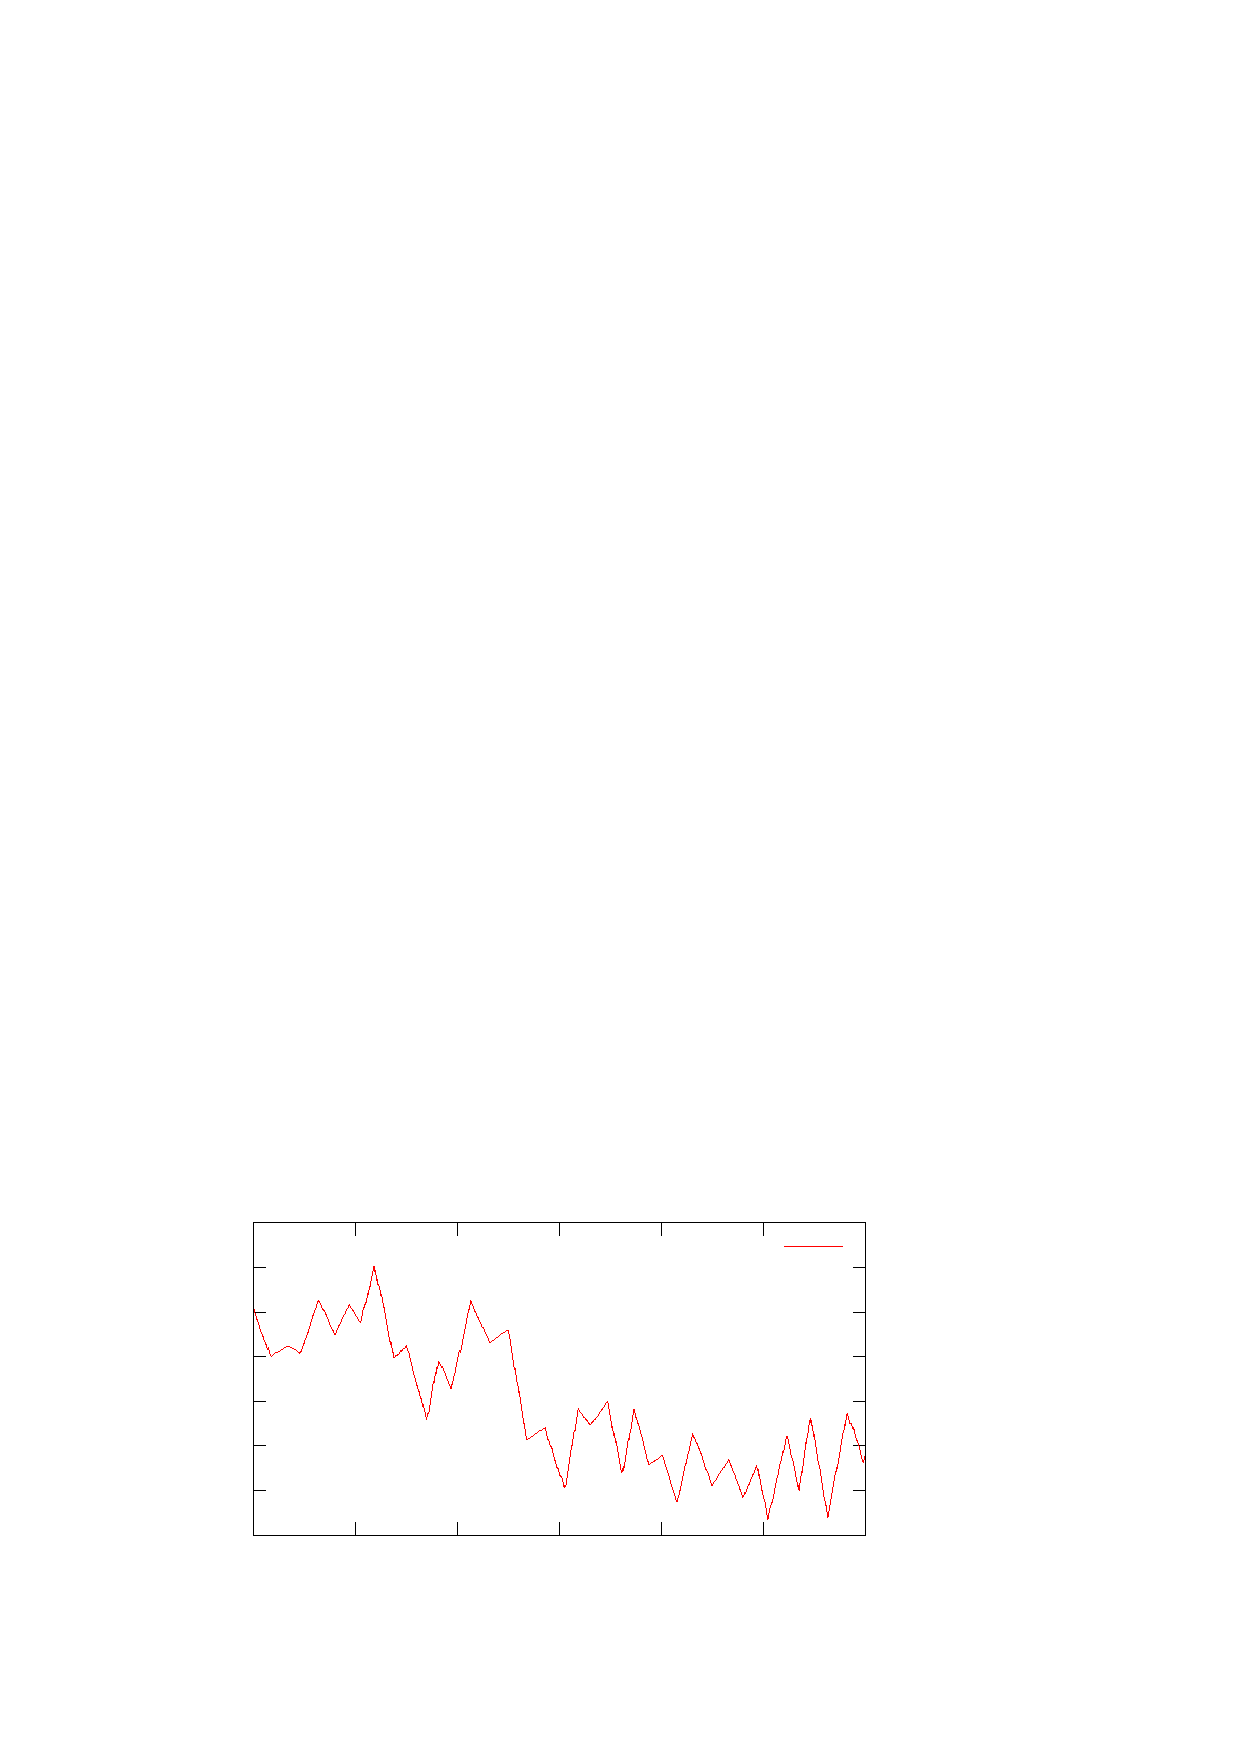
\includegraphics{inde-values}%
\end{picture}%
\begingroup
\setlength{\unitlength}{0.0200bp}%
\begin{picture}(18000,10800)(0,0)%
\put(2200,1650){\makebox(0,0)[r]{\strut{}-250}}%
\put(2200,2721){\makebox(0,0)[r]{\strut{}-200}}%
\put(2200,3793){\makebox(0,0)[r]{\strut{}-150}}%
\put(2200,4864){\makebox(0,0)[r]{\strut{}-100}}%
\put(2200,5936){\makebox(0,0)[r]{\strut{}-50}}%
\put(2200,7007){\makebox(0,0)[r]{\strut{} 0}}%
\put(2200,8079){\makebox(0,0)[r]{\strut{} 50}}%
\put(2200,9150){\makebox(0,0)[r]{\strut{} 100}}%
\put(2475,1100){\makebox(0,0){\strut{} 0}}%
\put(4925,1100){\makebox(0,0){\strut{} 500}}%
\put(7375,1100){\makebox(0,0){\strut{} 1000}}%
\put(9825,1100){\makebox(0,0){\strut{} 1500}}%
\put(12275,1100){\makebox(0,0){\strut{} 2000}}%
\put(14725,1100){\makebox(0,0){\strut{} 2500}}%
\put(17175,1100){\makebox(0,0){\strut{} 3000}}%
\put(550,5400){\rotatebox{90}{\makebox(0,0){\strut{}value}}}%
\put(9825,275){\makebox(0,0){\strut{}time step}}%
\put(9825,9975){\makebox(0,0){\strut{}increasing/decreasing method 4 sample plot}}%
\put(14950,8575){\makebox(0,0)[r]{\strut{}"inde-values.data"}}%
\end{picture}%
\endgroup
\endinput

\label{fig:inde4plot}
\caption{Increasing/decreasing method 4 sample plot.}
\end{figure}

\begin{figure}
%GNUPLOT: LaTeX picture with Postscript
\begin{picture}(0,0)%
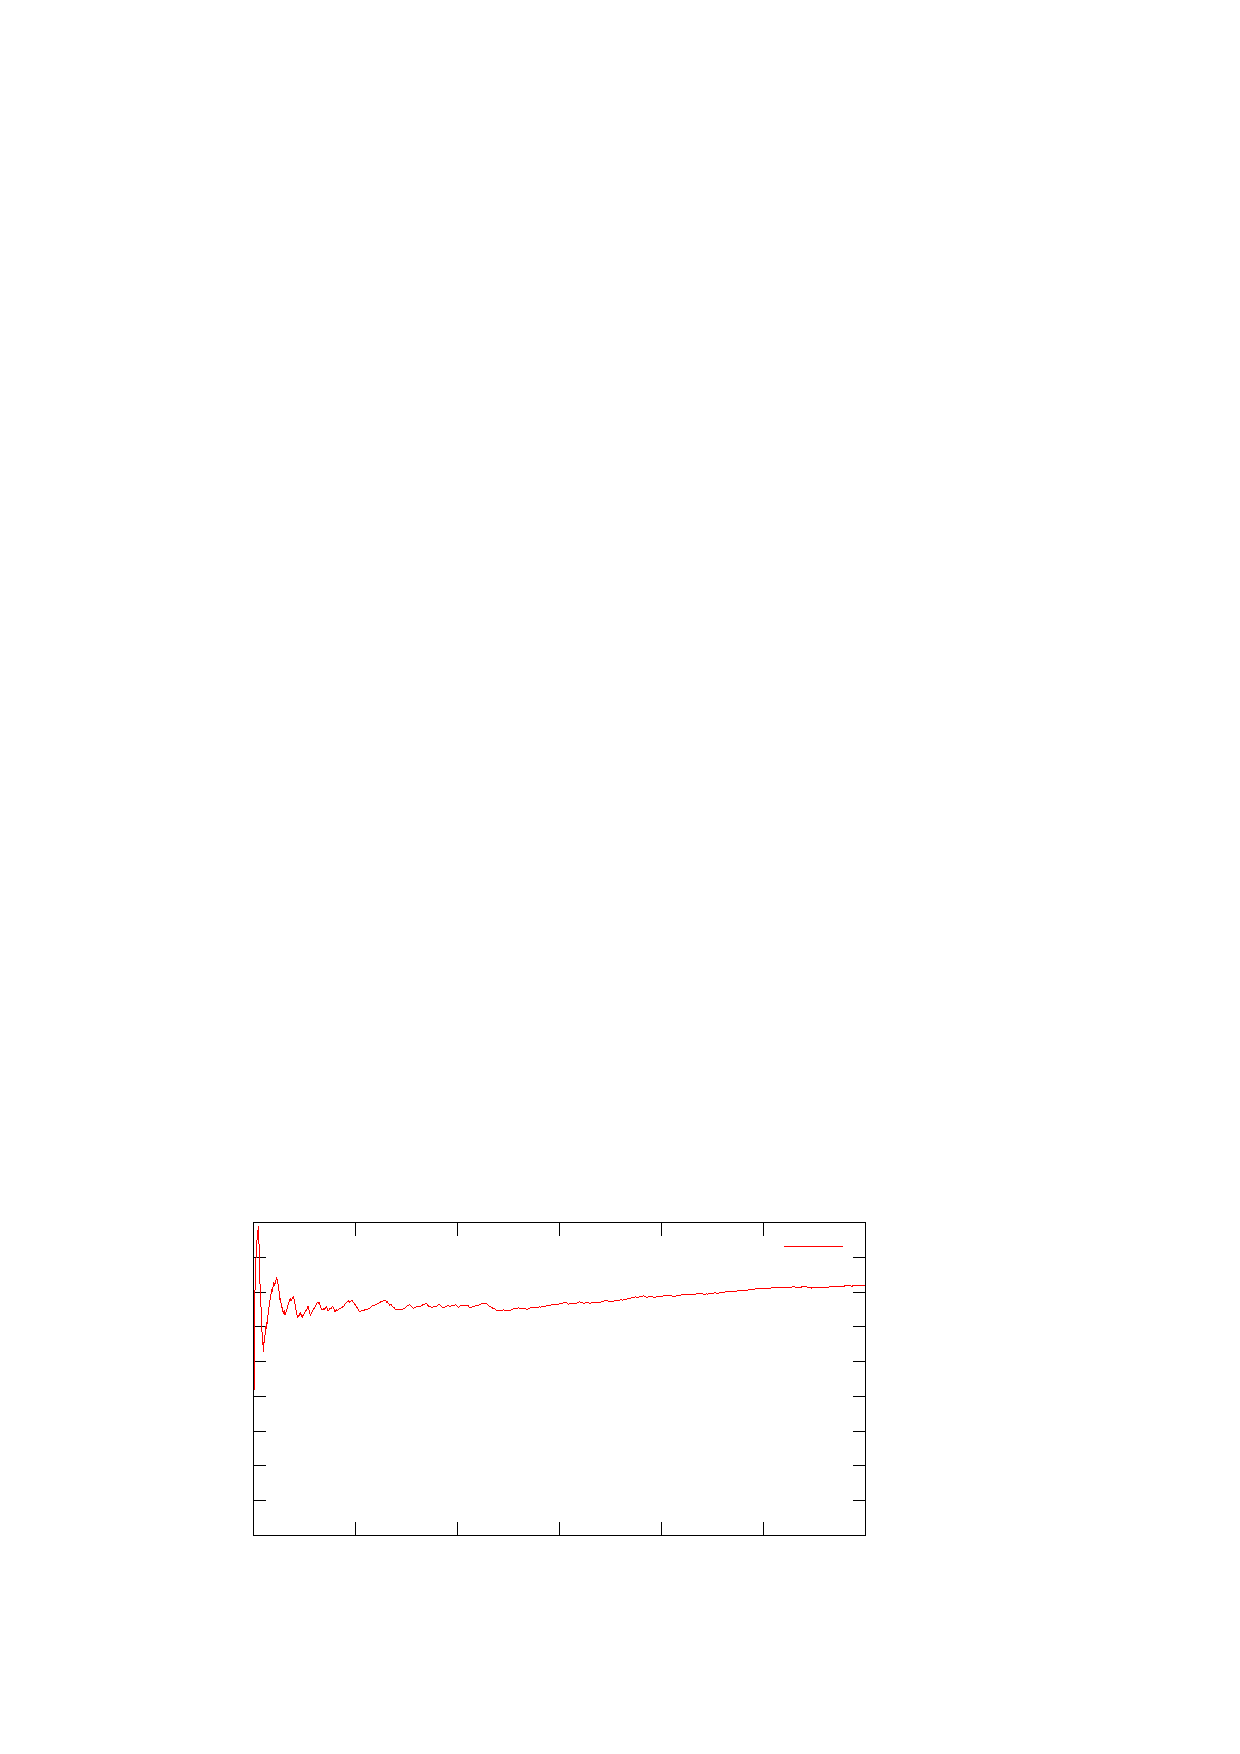
\includegraphics{inde-hist}%
\end{picture}%
\begingroup
\setlength{\unitlength}{0.0200bp}%
\begin{picture}(18000,10800)(0,0)%
\put(2200,1650){\makebox(0,0)[r]{\strut{} 0}}%
\put(2200,2483){\makebox(0,0)[r]{\strut{} 0.1}}%
\put(2200,3317){\makebox(0,0)[r]{\strut{} 0.2}}%
\put(2200,4150){\makebox(0,0)[r]{\strut{} 0.3}}%
\put(2200,4983){\makebox(0,0)[r]{\strut{} 0.4}}%
\put(2200,5817){\makebox(0,0)[r]{\strut{} 0.5}}%
\put(2200,6650){\makebox(0,0)[r]{\strut{} 0.6}}%
\put(2200,7483){\makebox(0,0)[r]{\strut{} 0.7}}%
\put(2200,8317){\makebox(0,0)[r]{\strut{} 0.8}}%
\put(2200,9150){\makebox(0,0)[r]{\strut{} 0.9}}%
\put(2475,1100){\makebox(0,0){\strut{} 0}}%
\put(4925,1100){\makebox(0,0){\strut{} 500}}%
\put(7375,1100){\makebox(0,0){\strut{} 1000}}%
\put(9825,1100){\makebox(0,0){\strut{} 1500}}%
\put(12275,1100){\makebox(0,0){\strut{} 2000}}%
\put(14725,1100){\makebox(0,0){\strut{} 2500}}%
\put(17175,1100){\makebox(0,0){\strut{} 3000}}%
\put(550,5400){\rotatebox{90}{\makebox(0,0){\strut{}accuracy}}}%
\put(9825,275){\makebox(0,0){\strut{}time step}}%
\put(9825,9975){\makebox(0,0){\strut{}increasing/decreasing method 4 sample performance}}%
\put(14950,8575){\makebox(0,0)[r]{\strut{}"inde-hist.data"}}%
\end{picture}%
\endgroup
\endinput

\label{fig:inde4perf}
\caption{Increasing/decreasing method 4 sample performance.}
\end{figure}

\subsection{The Stock Market}
\newcommand{\DJI}{\textasciicircum DJI}
We experimentally determined many of the parameters that are best for use on the stock market.
We used actual historical data of the Dow Jones Industrial Average (\DJI), with daily trading data starting on August 20, 1990, with data ending on August 18, 2006.
The data was gathered from Yahoo! Finance.
The first 100 data points of the time series were skipped, allowing for historical data that far back even in the very first day of simulated data, causing an actual start of analysis of January 11, 1991.
In each of these experiments, a statistical sample of at least 30 runs was gathered, each run going on for 1,500 simulated trading days (2,167 actual days, 5.93 years), for an end of December 16, 1996.
At each trading day the stock was given the option to either put all of its resources into the \DJI\ or into a bank account yielding roughly 4\% per annum.
The system initially had \$1,000,000.00.

In these trials we report:
\begin{enumerate}
\item the trial number,
\item the number of correct actions,
\item the percentage of correct actions,
\item the final financial return,
\item the ratio of the final financial return to that of the buy-and-hold strategy,
\item and the percentage returned per annum.
\end{enumerate}
We will use the buy-and-hold (B\&H) strategy as our primary performance benchmark.
In this strategy, the stock is purchased outright, and then the money is just left in the stock for the entire duration of the experiment.

\newenvironment{cgoreErt}[2]
{\begin{center}
   \begin{longtable}{|c|lrrlr|}
      \caption{#1}\label{#2}\remline\\
      \hline
      --- & \textbf{correct} & \textbf{\% correct} & \textbf{returns} & \textbf{B\&H ratio} & \textbf{\%pa}\\
      \hline
      B\&H & 806 & 53.733\% & \$2,745,309.50 & 1.0 & 18.54\%pa\\
      \hline
   \endfirsthead}
{\\ \hline\end{longtable}\end{center}}

Our initial parameters are listed in Table~\ref{tab:initial-parameters}, and were chosen by general trial and error throughout the software development process.

\begin{table}
\caption{Initial parameters for the TSC.}
\label{tab:initial-parameters}
\begin{tabular}{|r|l|}
   \hline
   \textbf{parameter} & \textbf{value} \\
   \hline
   max environment condition length & 10 \\
   valid operations & simple slope \\
   valid fields & closing price, opening price, and trading volume \\
   max total numerosity, $N$ & 400 \\
   learning rate, $\beta$ & 0.2 \\
   discount factor, $\gamma$ & 0.71 \\
   GA threshold, $\theta_{GA}$ & 25 \\
   equal error threshold, $\epsilon_0$ & 20.0 \\
   multiplier parameter, $\alpha$ & 0.1 \\
   crossover probability, $\chi$ & 0.8 \\
   mutation probability, $\mu$ & 0.04 \\
   exploration probability, $P_{explr}$ & 0.2 \\
   fitness fraction threshold, $\delta$ & 0.1 \\
   covering probability, $P_\#$ & 0.33 \\
   initial prediction, $p_I$ & 10.0 \\
   initial prediction error, $\epsilon_I$ & 0.0 \\
   initial fitness, $F_I$ & 0.01\\
   \hline
\end{tabular}
\end{table}

\subsubsection{Reward Methods}
Several different possible reward methods for use in the stock market were considered, and we analyzed their relative performance.
We refer to these different reward methods as $a_1$, $a_2$, $b$, $c$, $d_{opt}$, and $d_{pess}$.

Reward method $a_1$ is very simple:
\begin{algorithmic}[1]
\IF{the correct action is taken}
   \RETURN a reward of 1,000.
\ELSE
   \RETURN a reward of 0,
\ENDIF
\end{algorithmic}

It had the results as described in Table~\ref{tab:reward-a1} over 36 trials.

\begin{cgoreErt}{TSC results for reward method $a_1$.}{tab:reward-a1}
arith mean & 754 & 50.256\% & \$1,853,080.30 & 0.67500 & 10.96\%pa \\
std dev & 22.3 & 1.489\% & \$333,964.25 & 0.12165 & 1.98\%pa \\
max & 797 & 53.133\% & \$2,527,462.80 & 0.92065 & 16.91\%pa \\
min & 697 & 46.467\% & \$1,117,451.00 & 0.40704 & 1.89\%pa
\end{cgoreErt}

Reward method $a_2$ is almost identical to $a_1$:
\begin{algorithmic}[1]
\IF{the correct action is taken}
   \RETURN a reward of 1,000.
\ELSE
   \RETURN a reward of -200.
\ENDIF
\end{algorithmic}

It had the results as described in Table~\ref{tab:reward-a2} over 44 trials.

\begin{cgoreErt}{TSC results for reward method $a_2$.}{tab:reward-a2}
arith mean & 748 & 49.867\% & \$1,863,365.60 & 0.67875 & 11.06\%pa \\
std dev & 23.4 & 1.557\% & \$294,466.10 & 0.10726 & 1.75\%pa \\
max & 790 & 52.667\% & \$2,571,187.50 & 0.93657 & 17.25\%pa \\
min & 693 & 46.2\% & \$1,358,889.10 & 0.49499 & 5.31\%pa
\end{cgoreErt}

Reward method $b$ offers slightly more incentive for good-performing rules:
\begin{algorithmic}[1]
\LETARROW{$\$_{ratio}$, the money ratio} $\frac{\$_{t+1}}{\$_t}$, the ratio of the money the classifier has immediately one time-step in the future to the money it currently has.
\IF{$\$_{ratio} > 1.005$}
   \RETURN a reward of 1,000.
\ELSE
   \RETURN a reward of 0.
\ENDIF
\end{algorithmic}

It had the results as described in Table~\ref{tab:reward-b} over 57 trials.

\begin{cgoreErt}{TSC results for reward method $b$.}{tab:reward-b}
arith mean & 750 & 49.992\% & \$1,792,041.90 & 0.65276 & 10.33\%pa \\
std dev & 27.9\% & 1.8631344 & \$378,179.50 & 0.13775 & 2.18\%pa \\
max & 815 & 54.333\% & \$2,820,059.80 & 1.02723 & 19.09\%pa \\
min & 692 & 46.133\% & \$1,219,942.60 & 0.44437 & 3.41\%pa
\end{cgoreErt}

Reward method $c$ tries to scale the reward:
\begin{algorithmic}[1]
\LET $\$_{ratio}$ be the money ratio as previously defined.
\LETARROW{$m$} 1000, a multiplier.
\LETARROW{$e$} 2, an exponent.
\LETARROW{$s$} 1.015, a threshold term.
\RETURN $m \cdot (\$_{ratio}-s)^e$
\end{algorithmic}

It had the results as described in Table~\ref{tab:reward-c} over 30 trials.

\begin{cgoreErt}{TSC results for reward method $c$.}{tab:reward-c}
arith mean  & 747 & 49.791\% & \$1,795,971.30 & 0.65420 & 10.37\%pa \\
std dev & 20.2 & 1.345\% & \$300,842.88 & 0.10958 & 1.74\%pa \\
max & 790 & 52.667\% & \$2,407,121.50 & 0.87681 & 15.95\%pa \\
min & 702 & 46.8\% & \$1,340,345.30 & 0.48823 & 5.07\%pa
\end{cgoreErt}

\newpage
Reward method $d$ is slightly more complex than the rest:
\begin{algorithmic}[1]
\INPUT $cu$, the amount of reward if the classifier is correct on an up day.
\INPUT $cd$, the amount of reward if the classifier is correct on an down day.
\INPUT $iu$, the amount of reward if the classifier is incorrect on an up day.
\INPUT $id$, the amount of reward if the classifier is incorrect on an down day.
\COMMENT{Days that are not up are viewed as down days here.}
\IF{the classifier has chosen the correct action $\land$ it is an up day}
   \RETURN $cu$.
\ELSIF{the classifier has chosen the correct action $\land$ it is a down day}
   \RETURN $cd$.
\ELSIF{the classifier has chosen the incorrect action $\land$ it is an up day}
   \RETURN $iu$.
\ELSIF{the classifier has chosen the incorrect action $\land$ it is a down day}
   \RETURN $id$.
\ENDIF
\end{algorithmic}
From this we have the two reward methods $d_{opt}$, which is optimistic, and $d_{pess}$, which is pessimistic.

Reward method $d_{opt}$ calls $d$ with the values of $cu=1000, cd=750, iu=0, id=200$.
It had the results as described in Table~\ref{tab:reward-dopt} over 45 trials.

\begin{cgoreErt}{TSC results for reward method $d_{opt}$.}{tab:reward-dopt}
arith mean & 728 & 48.526\% & \$1,624,189.40 & 0.59162 & 8.52\%pa \\
std dev & 22.2 & 1.477\% & \$223,009.56 & 0.08123 & 1.17\%pa \\
max & 786 & 52.4\% & \$2,122,616.30 & 0.77318 & 13.52\%pa \\
min & 689 & 45.933\% & \$1,163,151.90 & 0.42369 & 2.58\%pa
\end{cgoreErt}

Reward method $d_{pess}$ calls $d$ with the values of $cu=750, cd=1000, iu=200, id=0$.
It had the results as described in Table~\ref{tab:reward-dpess} over 45 trials.

\begin{cgoreErt}{TSC results for reward method $d_{pess}$.}{tab:reward-dpess}
arith mean & 728 & 48.526\% & \$1,624,189.40 & 0.59162 & 8.52\%pa \\
std dev & 22.2\% & 1.477 & \$223,009.56 & 0.08123 & 1.17\%pa \\
max & 786 & 52.4\% & \$2,122,616.30 & 0.77318 & 13.52\%pa \\
min & 689 & 45.933\% & \$1,163,151.90 & 0.42369 & 2.58\%pa
\end{cgoreErt}

From these experiments we see that the $a$ methods are the best performing, although there is no effective difference between the performance of $a_1$ and $a_2$: this is because the scaling of the reward should not effect the outcome of the reward method at all.
We arbitrarily choose of the two to employ $a_2$ for the remaining experiments.


\subsubsection{GA Thresholds}
After deciding on $a_2$ as the best reward method and keeping it for the rest of these tests, we turn our attention to optimizing the GA threshold $\theta_{GA}$, which is described earlier in \S\ref{sec:ga-threshold}.
We chose to look at the possible values for this parameter of 25,  35, 45, and 50.

A GA threshold of 25 was used in the previous situation, so we can borrow the results from that $a_2$ run; refer to Table~\ref{tab:reward-a2}.

For a GA threshold value of 35, we observed the results as described in Table~\ref{tab:gathreshold35} over 30 trials.

\enlargethispage{2\baselineskip}
\begin{cgoreErt}{TSC results for a GA threshold of 35.}{tab:gathreshold35}
arith mean & 759 & 50.571\% & \$1,874,746.50 & 0.68289 & 11.17\%pa \\
std dev & 22.7 & 1.513\% & \$315,092.60 & 0.11477 & 1.88\%pa \\
max & 806 & 53.733\% & \$2,627,517.80 & 0.95709 & 17.68\%pa \\
min & 719 & 47.933\% & \$1,346,346.10 & 0.49042 & 5.14\%pa
\end{cgoreErt}

For a GA threshold value of 45, we observed the results as described in Table~\ref{tab:gathreshold45} over 31 trials.

\begin{cgoreErt}{TSC results for a GA threshold of 45.}{tab:gathreshold45}
arith mean & 760  & 50.688\% & \$1,881,119.10 & 0.68521 & 11.24\%pa \\
std dev    & 25.6 &  1.706\% &   \$217,843.06 & 0.07935 & 1.30\%pa \\
max        & 816  & 54.4\%   & \$2,297,796.00 & 0.83699 & 15.05\%pa \\
min        & 699  & 46.6\%   & \$1,250,916.30 & 0.45566 & 3.85\%pa
\end{cgoreErt}

For a GA threshold value of 50, we observed the results as described in Table~\ref{tab:gathreshold50} over 30 trials.

\begin{cgoreErt}{TSC results for a GA threshold of 50.}{tab:gathreshold50}
arith mean & 763 & 50.891\% & \$1,885,079.90 & 0.68665 & 11.28\%pa \\
std dev & 21.1 & 1.405\% & \$293,885.56 & 0.10705 & 1.76\%pa \\
max & 808 & 53.867\% & \$2,425,741.30 & 0.88359 & 16.10\%pa \\
min & 713 & 47.533\% & \$1,329,746.00 & 0.48437 & 4.91\%pa
\end{cgoreErt}

There was no significant effect on the results of the algorithm based on the GA threshold: all of the other means fall well within $1\over4$ of a standard deviation relative to the initial value of $\theta_{GA} = 25$, so we will employ that value for all remaining experiments.


\subsubsection{Crossover Probabilities}
After deciding on the correct reward method and the correct GA threshold, using those results, we investigated the crossover probability, which is described earlier in \S\ref{sec:crossover-probability}.
We chose to look at 0.5, 0.6, 0.7, 0.8, and 0.9.

For a crossover probability of $\chi = 0.3$, we obtained the results as described in Table~\ref{tab:chi0.3} over 33 trials.

\begin{cgoreErt}{TSC results for $\chi=0.3$.}{tab:chi0.3}
arith mean & 755 & 50.358\% & \$1,862,015.40 & 0.67825 & 11.05\%pa \\
std dev & 24.3 & 1.621\% & \$213,367.14 & 0.07772 & 1.27\%pa \\
max & 829 & 55.267\% & \$2,354,066.50 & 0.85749 & 15.52\%pa \\
min & 712 & 47.467\% & \$1,313,611.90 & 0.47849 & 4.71\%pa
\end{cgoreErt}

For a crossover probability of $\chi = 0.5$, we obtained the results as described in Table~\ref{tab:chi0.5} over 31 trials.

\begin{cgoreErt}{TSC results for $\chi=0.5$.}{tab:chi0.5}
arith mean & 754 & 50.275\% & \$1,882,082.30 & 0.68556 & 11.25\%pa \\
std dev & 24.9 & 1.662\% & \$265,281.13 & 0.09663 & 1.59\%pa \\
max & 799 & 53.267\% & \$2,426,894.30 & 0.88401 & 16.11\%pa \\
min & 717 & 47.8 & \$1,354,985.40 & 0.49356 & 5.25\%pa
\end{cgoreErt}

For a crossover probability of $\chi = 0.7$, we obtained the results as described in Table~\ref{tab:chi0.7} over 34 trials.

\begin{cgoreErt}{TSC results for $\chi=0.7$.}{tab:chi0.7}
arith mean & 754 & 50.275\% & \$1,884,173.30 & 0.68632 & 11.27\%pa \\
std dev & 28.9 & 1.930\% & \$258,017.90 & 0.09399 & 1.54\%pa \\
max & 809 & 53.933\% & \$2,526,742.80 & 0.92039 & 16.90\%pa \\
min & 688 & 45.867\% & \$1,264,236.40 & 0.46051 & 4.03\%pa
\end{cgoreErt}

A crossover probability of 0.8 was used in the previous situation, so we can borrow the results from the $\theta_{GA} = 25$ run; refer to Table~\ref{tab:reward-a2}.

For a crossover probability of $\chi = 0.9$, we obtained the results as described in Table~\ref{tab:chi0.9} over 39 trials.

\begin{cgoreErt}{TSC results for $\chi=0.9$.}{tab:chi0.9}
arith mean & 759 & 50.626\% & \$1,943,606.10 & 0.70797 & 11.85\% \\
std dev & 21.9 & 1.462\% & \$277,516.22 & 0.10109 & 1.69\%  \\
max & 801 & 53.400\% & \$2,399,683.00 & 0.87410 & 15.89\% \\
min & 707 & 47.133\% & \$1,419,889.40 & 0.51721 & 6.09\%
\end{cgoreErt}

We can now easily observe that a crossover probability of $\chi=0.9$ offers the best results with an arithmetic mean of 11.85\%pa, and we employ it for all of the remaining experiments.


\subsubsection{Mutation Probabilities}
Using all of our previous results, we then looked into the mutation probability, described earlier in \S\ref{sec:mutation-probability}.
We looked at values of 0.04, 0.06, 0.08, 0.10, 0.15, and 0.20.

A mutation probability $\mu=0.04$ was used in the previous situation, so we can borrow the results from the $\chi = 0.9$ run; refer to Table~\ref{tab:chi0.9}.

For a mutation probability $\mu=0.06$, we observed the results as described in Table~\ref{tab:mu0.06} over 34 trials.

\begin{cgoreErt}{TSC results for $\mu=0.06$.}{tab:mu0.06}
arith mean & 762 & 50.831\% & \$1,972,095.00 & 0.71835 & 12.13\%pa \\
std dev & 21.5 & 1.433\% & \$255,299.13 & 0.09299 & 1.57\%pa \\
max & 792 & 52.800\% & \$2,734,496.80 & 0.99606 & 18.47\%pa \\
min & 704 & 46.933\% & \$1,579,600.50 & 0.57538 & 8.01\%pa
\end{cgoreErt}

For a mutation probability $\mu=0.08$, we observed the results as described in Table~\ref{tab:mu0.08} over 39 trials.

\begin{cgoreErt}{TSC results for $\mu=0.08$.}{tab:mu0.08}
arith mean & 754 & 50.285\% & \$1,905,925.10 & 0.69425 & 11.48\%pa \\
std dev & 29.79326 & 1.986\% & \$285,127.30 & 0.10386 & 1.72\%pa \\
max & 806 & 53.733\% & \$2,421,790.30 & 0.88216 & 16.07\%pa  \\
min & 668 & 44.533\% & \$1,230,840.30 & 0.44834 & 3.56\%pa
\end{cgoreErt}

For a mutation probability $\mu=0.10$, we observed the results as described in Table~\ref{tab:mu0.10} over 36 trials.

\begin{cgoreErt}{TSC results for $\mu=0.10$.}{tab:mu0.10}
arith mean & 761 & 50.744\% & \$1,950,889.10 & 0.71063 & 11.92\%pa \\
std dev & 22.6 & 1.506\% & \$299,845.56 & 0.10922 & 1.83\%pa \\
max & 796 & 53.067\% & \$2,891,320.00 & 1.05319 & 19.59\%pa \\
min & 709 & 47.267\% & \$1,250,508.00 & 0.45551 & 3.84\%pa
\end{cgoreErt}

For a mutation probability $\mu=0.15$, we observed the results as described in Table~\ref{tab:mu0.15} over 32 trials.

\begin{cgoreErt}{TSC results for $\mu=0.15$.}{tab:mu0.15}
arith mean & 763 & 50.908\% & \$2,037,007.90 & 0.74200 & 12.74\%pa \\
std dev & 22.299\% & 1.487\% & \$320,506.80 & 0.11675 & 2.00\%pa \\
max & 804 & 53.600\% & \$2,975,396.80 & 1.08381 & 20.17\%pa \\
min & 719 & 47.933\% & \$1,406,036.50 & 0.51216 & 5.91\%pa
\end{cgoreErt}

For a mutation probability $\mu=0.20$, we observed the results as described in Table~\ref{tab:mu0.20} over 36 trials.

\enlargethispage{2\baselineskip}
\begin{cgoreErt}{TSC results for $\mu=0.20$.}{tab:mu0.20}
arith mean & 762 & 50.800\% & \$1,889,297.80 & 0.68819 & 11.42\%pa \\
std dev & 24.369835 & 1.625\% & \$232,916.92 & 0.08484 & 1.40\%pa \\
max & 803 & 53.533\% & \$2,708,086.00 & 0.98644 & 18.28\%pa \\
min & 697 & 46.467\% & \$1,502,196.10 & 0.54719 & 7.10\%pa
\end{cgoreErt}

We can now easily observe that a mutation probability of $\mu=0.15$ offers the best results with a arithmetic mean of 12.74\%pa, and we therefore use that value for all remaining experiments.


\subsubsection{Exploration Probabilities}
After this we looked at the exploration probability, which we describe in \S\ref{sec:exploration-probability}.
We investigated the possible values of 0.1, 0.2, 0.3, and 0.4, using our previous results for the rest of the parameters.

For an exploration probability of $P_{explr}=0.1$, we observed the results as described in Table~\ref{tab:pexplr0.1} over 42 trials.

\begin{cgoreErt}{TSC results for $P_{explr}=0.1$.}{tab:pexplr0.1}
arith mean & 762 & 50.795\% & \$1,849,187.80 & 0.67358 & 10.92\%pa \\
std dev & 28.9 & 1.925\% & \$233,230.42 & 0.08496 & 1.38\%pa \\
max & 810 & 54.000\% & \$2,446,262.50 & 0.89107 & 16.27\%pa \\
min & 691 & 46.067\% & \$1,210,933.40 & 0.44109 & 3.28\%pa
\end{cgoreErt}

An exploration probability of $P_{explr}=0.2$ was used in the previous situation, so we can borrow the results from the $\mu=0.15$ run; refer to Table~\ref{tab:mu0.15}.

\begin{cgoreErt}{TSC results for $P_{explr}=0.15$.}{tab:pexplr0.15}
\hline
arith mean & 763 & 50.908\% & \$2,037,007.90 & 0.74200 & 12.74\%pa \\
std dev & 22.3 & 1.487\% & \$320,506.80 & 0.11675 & 2.00\%pa \\
max & 804 & 53.600\% & \$2,975,396.80 & 1.08381 & 20.17\%pa \\
min & 719 & 47.933\% & \$1,406,036.50 & 0.51216 & 5.91\%pa
\end{cgoreErt}

For an exploration probability of $P_{explr}=0.3$, we observed the results as described in Table~\ref{tab:pexplr0.3} over 40 trials.

\begin{cgoreErt}{TSC results for $P_{explr}=0.3$.}{tab:pexplr0.3}
arith mean & 765 & 50.985\% & \$2,090,409.40 & 0.76145 & 13.23\%pa \\
std dev & 22.8 & 1.521\% & \$295,592.78 & 0.10768 & 1.87\%pa \\
max & 817 & 54.467\% & \$2,848,646.30 & 1.03764 & 19.29\%pa \\
min & 725 & 48.333\% & \$1,536,175.30 & 0.55956 & 7.50\%pa
\end{cgoreErt}

For an exploration probability of $P_{explr}=0.4$, we observed the results as described in Table~\ref{tab:pexplr0.4} over 47 trials.

\begin{cgoreErt}{TSC results for $P_{explr}=0.4$.}{tab:pexplr0.4}
arith mean & 767 & 51.119\% & \$1,950,627.60 & 0.71053 & 11.92\%pa \\
std dev & 19.5 & 1.299\% & \$196,644.44 & 0.07163 & 1.20\%pa \\
max & 806 & 53.733\% & \$2,395,224.50 & 0.87248 & 15.86\%pa \\
min & 730 & 48.667\% & \$1,637,668.40 & 0.59653 & 8.67\%pa
\end{cgoreErt}

We can now easily observe that an exploration probability of $P_{explr}=0.3$ offers the best results with an arithmetic mean of 13.23\%pa, and we therefore use that value.


%\subsubsection{Maximum Environment Condition Lengths}
%Using all of the parameters we have discovered so far, we look now at how different maximum environment condition lengths, which we describe in \S\ref{sec:maximum-environment-condition-length}, can affect the outcome.
%We tested 1, 2, 5, 10, and 20.

%\subsubsection{Maximum Temporal Mutations}
%After all of this, still accumulating good parameters and using them for this test as well, we investigated the maximum temporal mutation, which we describe earlier in \S\ref{sec:maximum-temporal-mutation}.
%We looked at this value at 1, 2, 5, 8, and 10.

%\subsubsection{Maximum Position Mutations}
%Finally, with all of the previous parameters decided, we investigated the maximum position mutation, which we describe in \S\ref{sec:maximum-position-mutation}.
%We looked at 1, 2, 5, 8, and 10.

\section{Conclusions and Final Results}
After all of our tests we arrived at the set of parameters in Table~\ref{tab:final-parameters} for the time series classifier.
In this table the return is the equivalent percentage per-year (\%pa) return provided by the parameters at that setting, and the B\&H ratio is the performance relative to a simplistic buy-and-hold stategy, with 1.0 being equal, less than 1.0 implying an underperforming result over the same period, and greater than 1.0 implying a superior result over the same time period.
The DJIA returned 18.54\%pa over the period investigated here, and we failed to meet that in any of our tests.
For example, 11.06\%pa implies that with all of the other parameters set to their initial default and the reward method set to $a_2$ is equivalent to a savings account yielding 11.06\%pa returns, but underperforming the DJIA itself if we were to merely buy and hold it for the same period of time.
While these results demonstrate the system's ability to learn a complex situation, they are not at a level acceptable for real-world use on the stock market, underperforming the simplistic buy-and-hold strategy.
Instead this system in its current form will only truly be applicable to less interesting problem spaces.

\begin{table}
\begin{center}
\caption{TSC Final Parameters}
\begin{tabular}{|r|l|rr|}
   \hline
   \textbf{parameter} & \textbf{value} & \textbf{return} & \textbf{B\&H ratio}\\
   \hline
   reward method & $a_2$ & 11.06\%pa & 0.67875 \\
   GA threshold, $\theta_{GA}$ & 25 & $\cdots$ & $\cdots$ \\
   crossover probability, $\chi$ & 0.9 & 11.85\%pa & 0.70797 \\
   mutation probability, $\mu$ & 0.15 & 12.74\%pa & 0.74200 \\
   exploration probability, $P_{explr}$ & 0.3 & 13.23\%pa & 0.76145\\
   \hline
\end{tabular}
\label{tab:final-parameters}
\end{center}
\end{table}

TSC would not be a usable real-world system for the stock market unless it were to result in returns in excess of the buy-and-hold strategy, which it did not.
If it were capable of outperforming buy-and-hold then we could use it for automated and unsupervised trading.
As it is, a more effective real-world approach would be to simply purchase an indexing fund.
TSC is no longer useful to us since our interest is specifically automated stock trading, and our research will continue towards other avenues of automated time series analysis and prediction, probably still in the area of evolutionary computation and possibly employing a novel type of LCS.

There are many real-world applications comprising simpler time series than the stock market, and TSC does have a lot of room left to grow still, so continued research by others would be welcomed and potentially fruitful.
TSC demonstrates that an LCS can natively represent a time series under analysis and learn in such an environment:
that demonstration is the most valuable result of this research, perhaps encouraging more attempts at LCS-based time series analysis methods.

\section{Future Work}
There are several opportunities for improvement on TSC.
Some of these are obvious and result from known simplifications and limitations of the current TSC system.
The most obvious paths for future research with this TSC fall into the following major tasks:
\begin{enumerate}
\item using more advanced $\phi$'s,
\item using more advanced $\omega$'s,
\item finishing the implementation of multidimensionality,
\item using more advanced concepts in the GA,
\item represent the rule strengths with polynomials instead of reals,
\item changing from a Michigan to a Pittsburg approach,
\item using a GP instead of a GA,
\item and applying the system to other real-world problems.
\end{enumerate}

Using more advanced $\phi$'s, is the most straightforward to start on.
In the version of TSC as outlined here, and in the associated code, it is entirely possible to use any lexical closure as a $\phi$, as long as it is capable of operating on one position of the time series data.
In our use we only used $\phi$ to select the data field, but there is no reason why this should not or could not have vastly more complex operations.
Any operations that would be useful in discernment might be useful.

Using more advanced $\omega$'s would address what is probably the greatest weakness of the current system.
At present we have only used a simple slope function for the $\omega$ and have not attempted anything else.
There are bound to be many more useful functions available.
We specifically expect that the ability to match against polynomials and against periodic functions would be of the most intrinsic value.

Extending TSC so that it is a system fully capable of handling multivariate time series depends on the previous two tasks' completion first.
The TSC system as described and the code used were both originally designed to handle multivariate time series, and therefore much of the work is already completed, but exactly what else remains to be finished is not entirely clear.
We assert that at least new $\omega$'s that are designed with multivariate time series in mind would be required, but there may be other elements of the TSC system that need revision as well.

Using more advanced concepts within TSC's GA would be one of the easiest methods of improvement.
The form of crossover we used was simple one-point crossover, and there are several well-known forms of crossover with better performance in general use.
Employing a self-adaptive GA to evolve its own parameters encoded in its gene could also provide for some major gains, as this has been the most computationally intensive part of our investigation.
Other methods of mutation may be beneficial, although this would require novel work: the non-standard form of the individuals in TSC appears to necessitate non-standard mutation approaches.
The easiest modification of the mutation that would possibly be beneficial would be to try a Gaussian form of mutation which would allow for more drastic alteration to the population members on rare occasions.
This would allow the system to adapt more fully to notably different environments.

The measures of the strengths here are real numbers currently, but we suspect that they may be better represented by polynomials, especially in the stock market problem since there is a great deal of difference in the value of a rule in differing times for any specific stock.

XCS and company use the so-called Michagan approach, where the entire population is the rule set.
We suspect that the Pittsburgh approach, where each individual in the population is a complete rule set, could possibly be a better fit for our stock market problem in specific and possibly time series problems in general.
This would be quite involved, and almost a complete redesign of the system.

Replacing the GA with a genetic program (GP), would be quite an undertaking.
This would allow for vastly more complex classification rules and could possibly discover new basic metrics for the time series problems presented to the system.
This would be of particular value with the stock market even though there are several well-known metrics because they are  rarely of any quality.
This would even more valuable for less-investigated time series problems since there might not even be any known metrics as of yet for the problem.

\enlargethispage{2\baselineskip}
The final task is actually many tasks: TSC should be applied to many more real-world problems, both to better solve those problems and to improve TSC itself.
We hope that this work will prove useful in many problems and look forward to its use by others.

% Leave the following two lines alone:
\appendix            % This command is used only once!
                     % It resets the formatting for the appendices.
%\printindex
%%%%%%%%%%%%%%%%%%%%%%%%%%%%%%%%%%%%%%%%%%%%%%%%%%%%%%%%%%%%%%%%%%%%
%                                                                 %
%                            APPENDIX A                           %
%                                                                 %
%%%%%%%%%%%%%%%%%%%%%%%%%%%%%%%%%%%%%%%%%%%%%%%%%%%%%%%%%%%%%%%%%%%
 
\section{THIS IS AN APPENDIX}
This is a sentence to take up space and look like text.
This is a sentence to take up space and look like text.
This is a sentence to take up space and look like text.
This is a sentence to take up space and look like text.
This is how equations are numbered in an appendix:
\begin{equation}
x^2 + y^2 = z^2
\end{equation} 
This is a sentence to take up space and look like text.
This is a sentence to take up space and look like text.
This is a sentence to take up space and look like text.
 
This is a sentence to take up space and look like text.
This is a sentence to take up space and look like text.
This is a sentence to take up space and look like text.
This is a sentence to take up space and look like text.
This is a sentence to take up space and look like text. 
    % appendix A
%%%%%%%%%%%%%%%%%%%%%%%%%%%%%%%%%%%%%%%%%%%%%%%%%%%%%%%%%%%%%%%%%%%%
%                                                                 %
%                            APPENDIX B                           %
%                                                                 %
%%%%%%%%%%%%%%%%%%%%%%%%%%%%%%%%%%%%%%%%%%%%%%%%%%%%%%%%%%%%%%%%%%%
 
\section{THIS IS ANOTHER APPENDIX}
This is a sentence to take up space and look like text.
This is a sentence to take up space and look like text.
This is a sentence to take up space and look like text.
This is a sentence to take up space and look like text.
This is how equations are numbered in another appendix:
\begin{equation}
\int\!\!\int z\,dx\,dy
\end{equation} 
This is a sentence to take up space and look like text.
This is a sentence to take up space and look like text.
This is a sentence to take up space and look like text.
\begin{equation}
\int\!\!\int z^{2xy}\,dx\,dy
\end{equation} 

This is a sentence to take up space and look like text.
This is a sentence to take up space and look like text.
This is a sentence to take up space and look like text.
This is a sentence to take up space and look like text.
This is a sentence to take up space and look like text. 
    % appendix B

%\end{doublespace}

\specialhead{BIBLIOGRAPHY}
\remline
\singlespace
%\bibliographystyle{ieeetr} 
\bibliographystyle{unsrt} 
\bibliography{thesis} 

\doublespace
\specialhead{VITA}
Christopher Mark Gore was born in Cleveland, Ohio, on December 8, 1978.
He received his High School Diploma from Triad High School in Saint Jacob, Illinois in 1997.
Then he received his Associate of Science from Southwestern Illinois College, located in Belleville, Illinois, in 2001.
After this he received his Bachelor of Science in Mathematics and Computer Science from Eastern Illinois University, located in Charleston, Illinois, in 2003.
This thesis is part of the requirements for the completion of his Master of Science in Computer Science from the Missouri University of Science and Technology, located in Rolla, Missouri, in 2008.
His computational interests include evolutionary algorithms and other methods of unaided computational learning, financial simulation and analysis, and Lisp.
His interest in investing is being actively and successfully engaged, but without the aid of the computational analysis presented here.
He is currently employed at Astronautics Corporation of America developing software for the Integrated Network Server Unit (INSU) that will fly with the Airbus~A400M, a large turboprop-driven military cargo aircraft designed to replace the aging C-130~Hercules throughout the world.
He married Monica Louise Gore (n\'ee Smith) on May 27, 2006, and they currently reside in Oak Creek, Wisconsin, a suburb of Milwaukee, with their cat Casper.


\end{document}
